\chapter{RESULTADOS E DISCUSSÃO}
\section{Resultados}
\subsection{Caso Base}

A Figura \ref{fig:t_padr_vels} apresenta o perfil de velocidades para o caso base, no qual evidencia-se o comportamento compensador do sistema e uma oscilação de alta frequência, artefato da resposta da FMINCON. A amplitude das oscilações tende a ser menor conforme exista uma maior resolução na interpolação do tempo, ou seja, apresente $dt$ menor. Ademais, conforme mencionado na seção anterior, o arranque foi restringido afim de controlar a amplitude dessas oscilações. %%COMPLEMENTAR

% Podemos observar os resultados das curvas geradas pelo Caso utilizando os parâmetros referência nas figuras
% \ref{fig:t_padr_vels}, \ref{fig:t_padr_des} e \ref{fig:t_padr_pos}. Nelas temos o comportamento compensador,
% especialmente nas curvas que tem o tempo como abicissa.
% Notamos também, principalmente na figura \ref{fig:t_padr_vels} uma ocilação de alta frequência que é um artefato
% da resposta da FMINCON, essa ocilação se encontrava em amplitude muito maior e foi controlada através de restrições quanto ao 
% arranque, ou seja, a mudança da aceleração no tempo.

\begin{figure}[H]
    \begin{center}
    \caption{Caso referência - Comportamento no tempo das velocidades em x e y da ponta e da referência}
    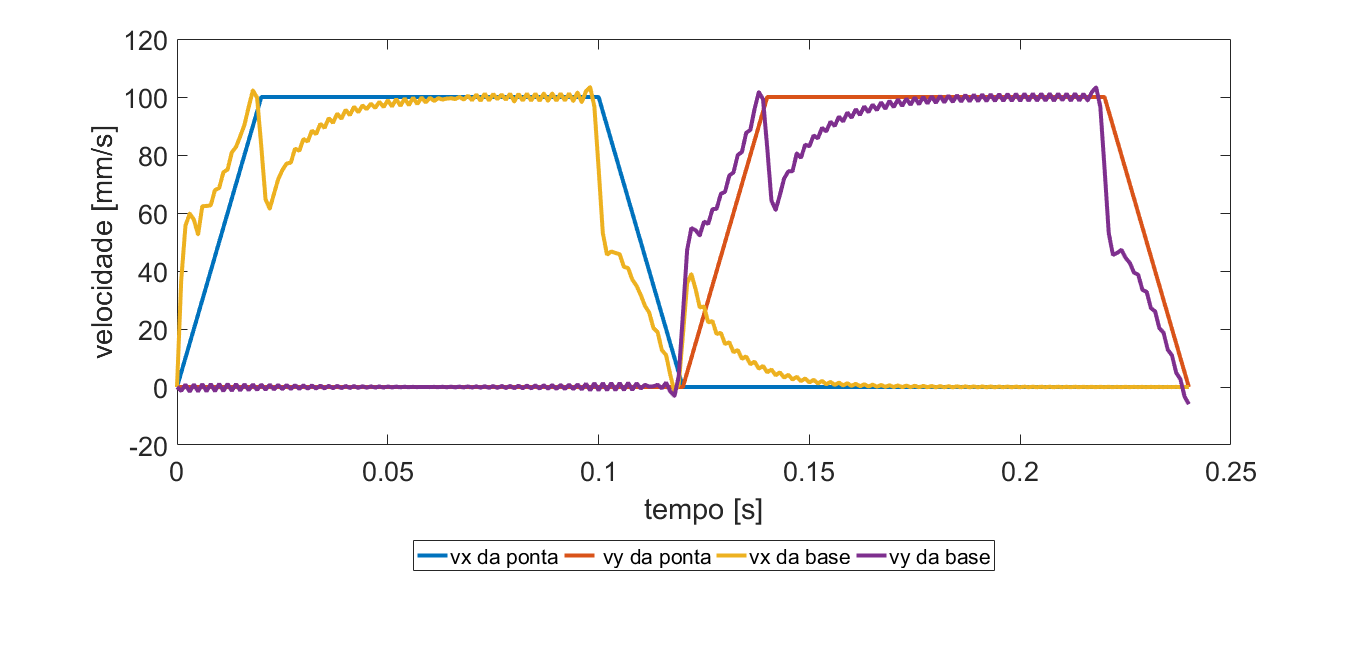
\includegraphics[scale=0.44]{Teste Padrao vels}
    \label{fig:t_padr_vels}
    \end{center}
\end{figure}

A Figura \ref{fig:t_padr_des} ...

\begin{figure}[H]
    \begin{center}
    \caption{Caso referência - Comportamento no tempo dos deslocamentos em x e y da ponta e da referência}
    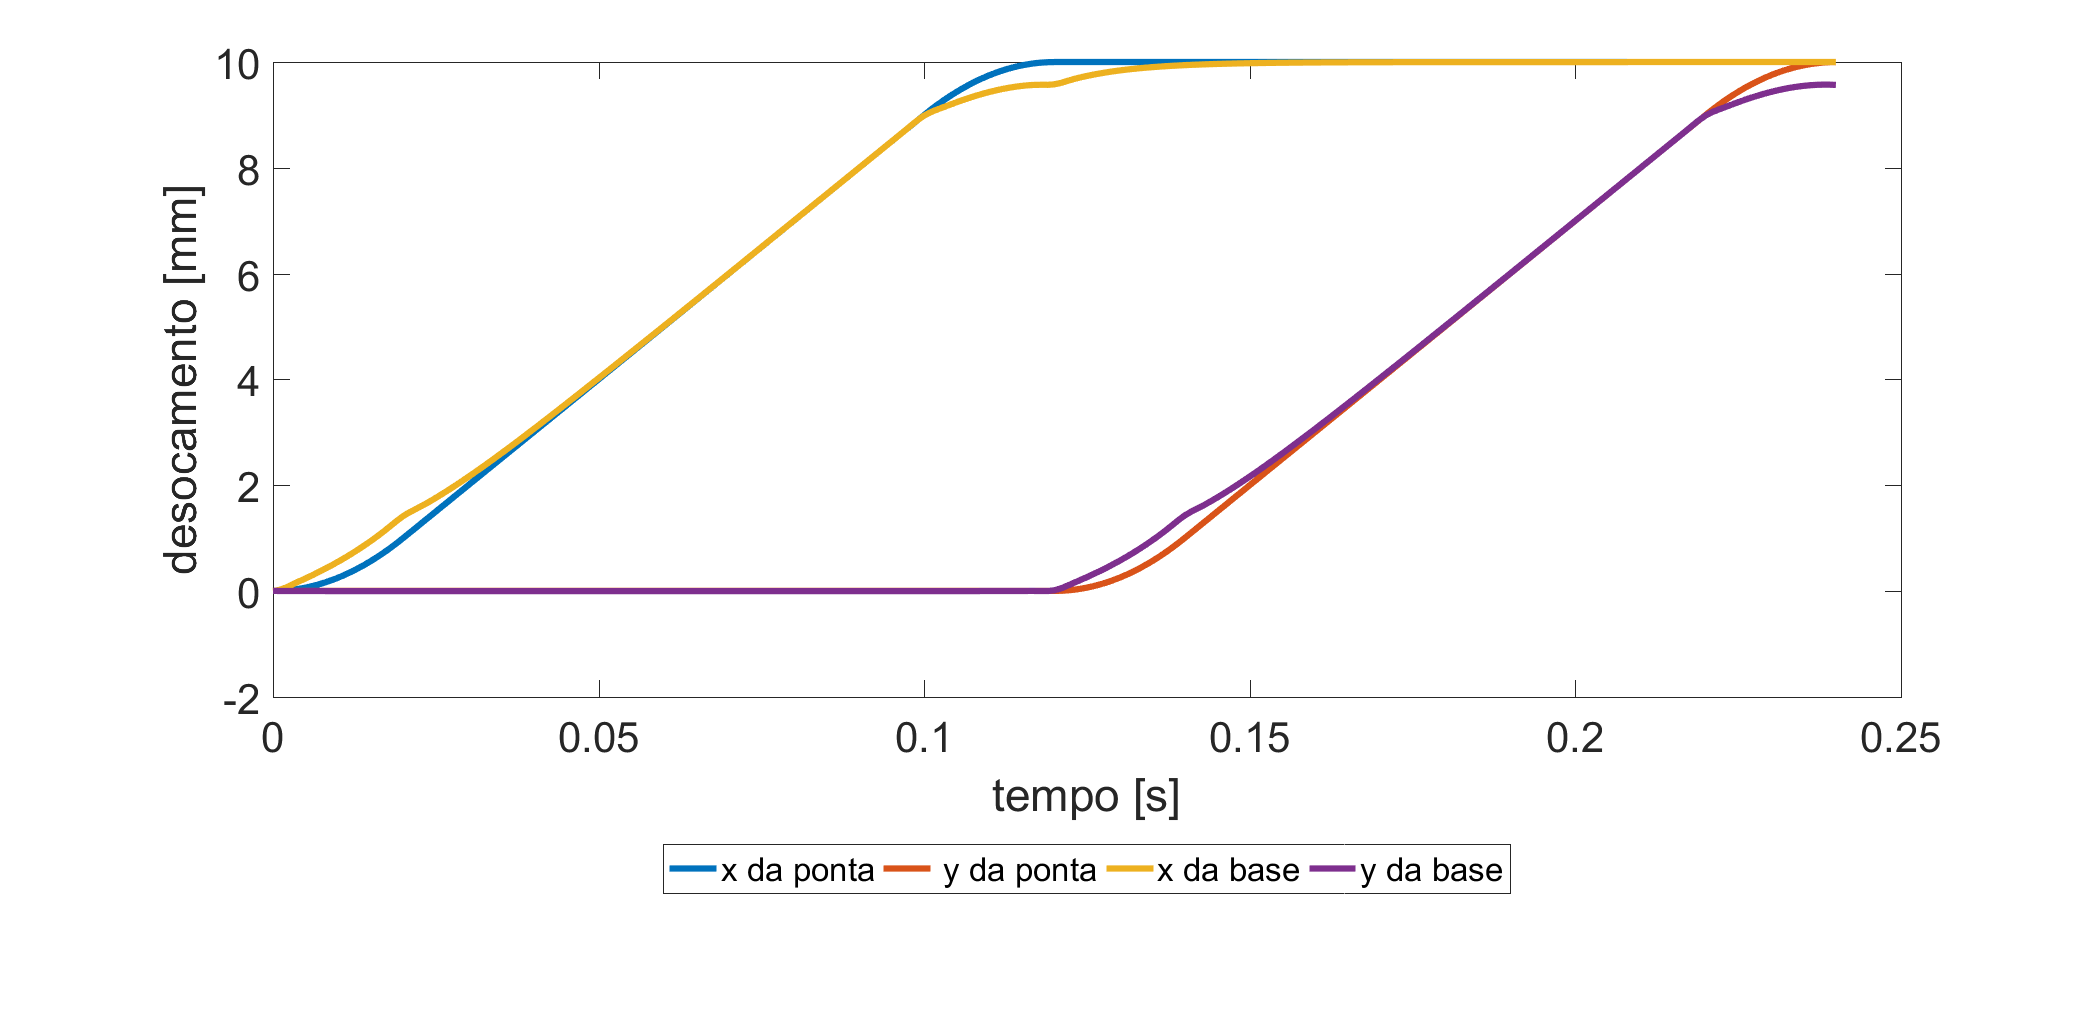
\includegraphics[scale=0.44]{Teste Padrao des}
    \label{fig:t_padr_des}
    \end{center}
\end{figure}

\begin{figure}[H]
    \begin{center}
    \caption{Caso referência - Caminho percorrido x vs y da ponta e da referência}
    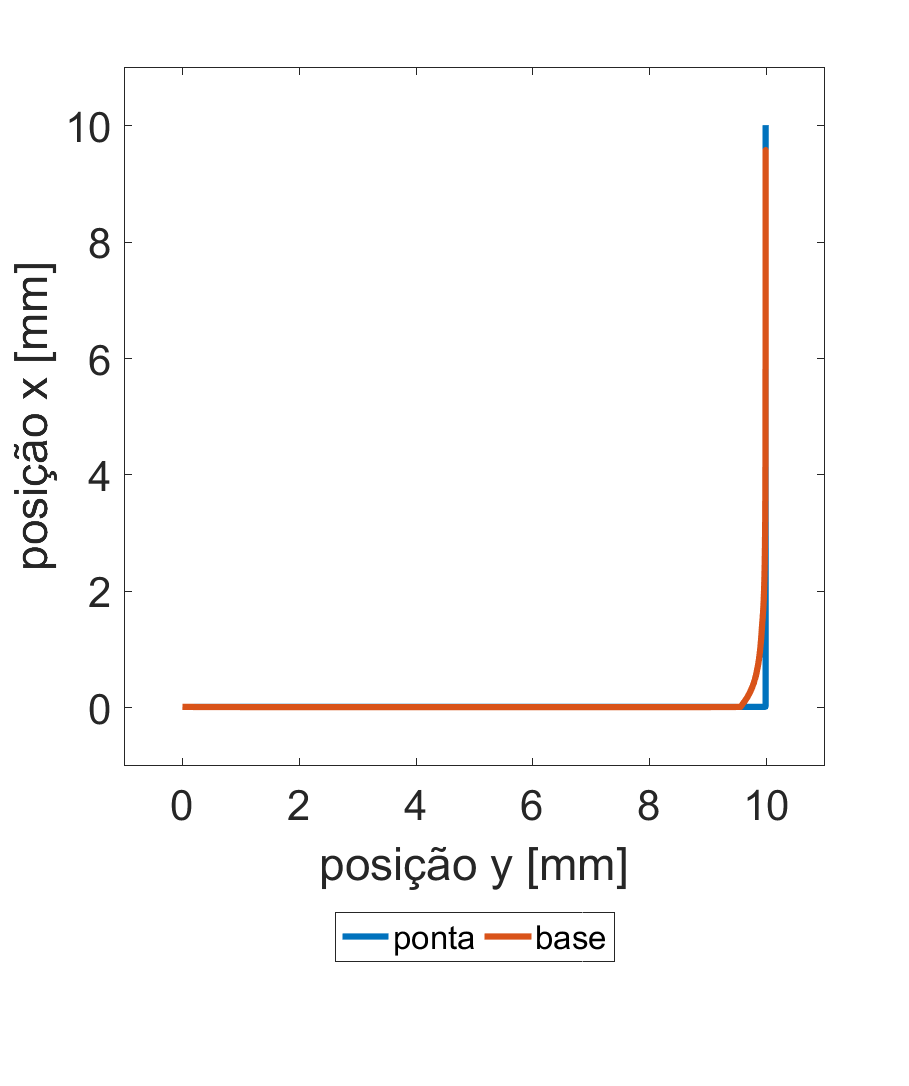
\includegraphics[scale=0.44]{Teste Padrao pos}
    \label{fig:t_padr_pos}
    \end{center}
\end{figure}

No gráfico da figura \ref{fig:t_padr_viab} nos indica a progressção das iterações da FMINCON, sendo cada
ponto uma iteração diferente, possuindo um valor correspondete ao número de vezes em que a função objetivo e as restrições foi avaliada
no eixo x e o valor da viabilidade, que como comentado na seção de metodologia, indica o maior valor de restrição não cumprido.
Podemos perceber o processo de convergência no decorrer das iterações, o que costuma indicar uma rodada de sucessos.
Percebe-se também que os níveis inicias da viabilidade ficam próximos de $7,5x10^3$, que foram niveis próximos na maioria dos Casos.
Por fim, temos que o tempo elapsado de simulação para este Caso foi de $89,8$ segundos, com os vetores de posição possuindo
um tamanho de 241 elementos.

\begin{figure}[H]
    \begin{center}
    \caption{Caso referência - Num de fun x Viabilidade}
    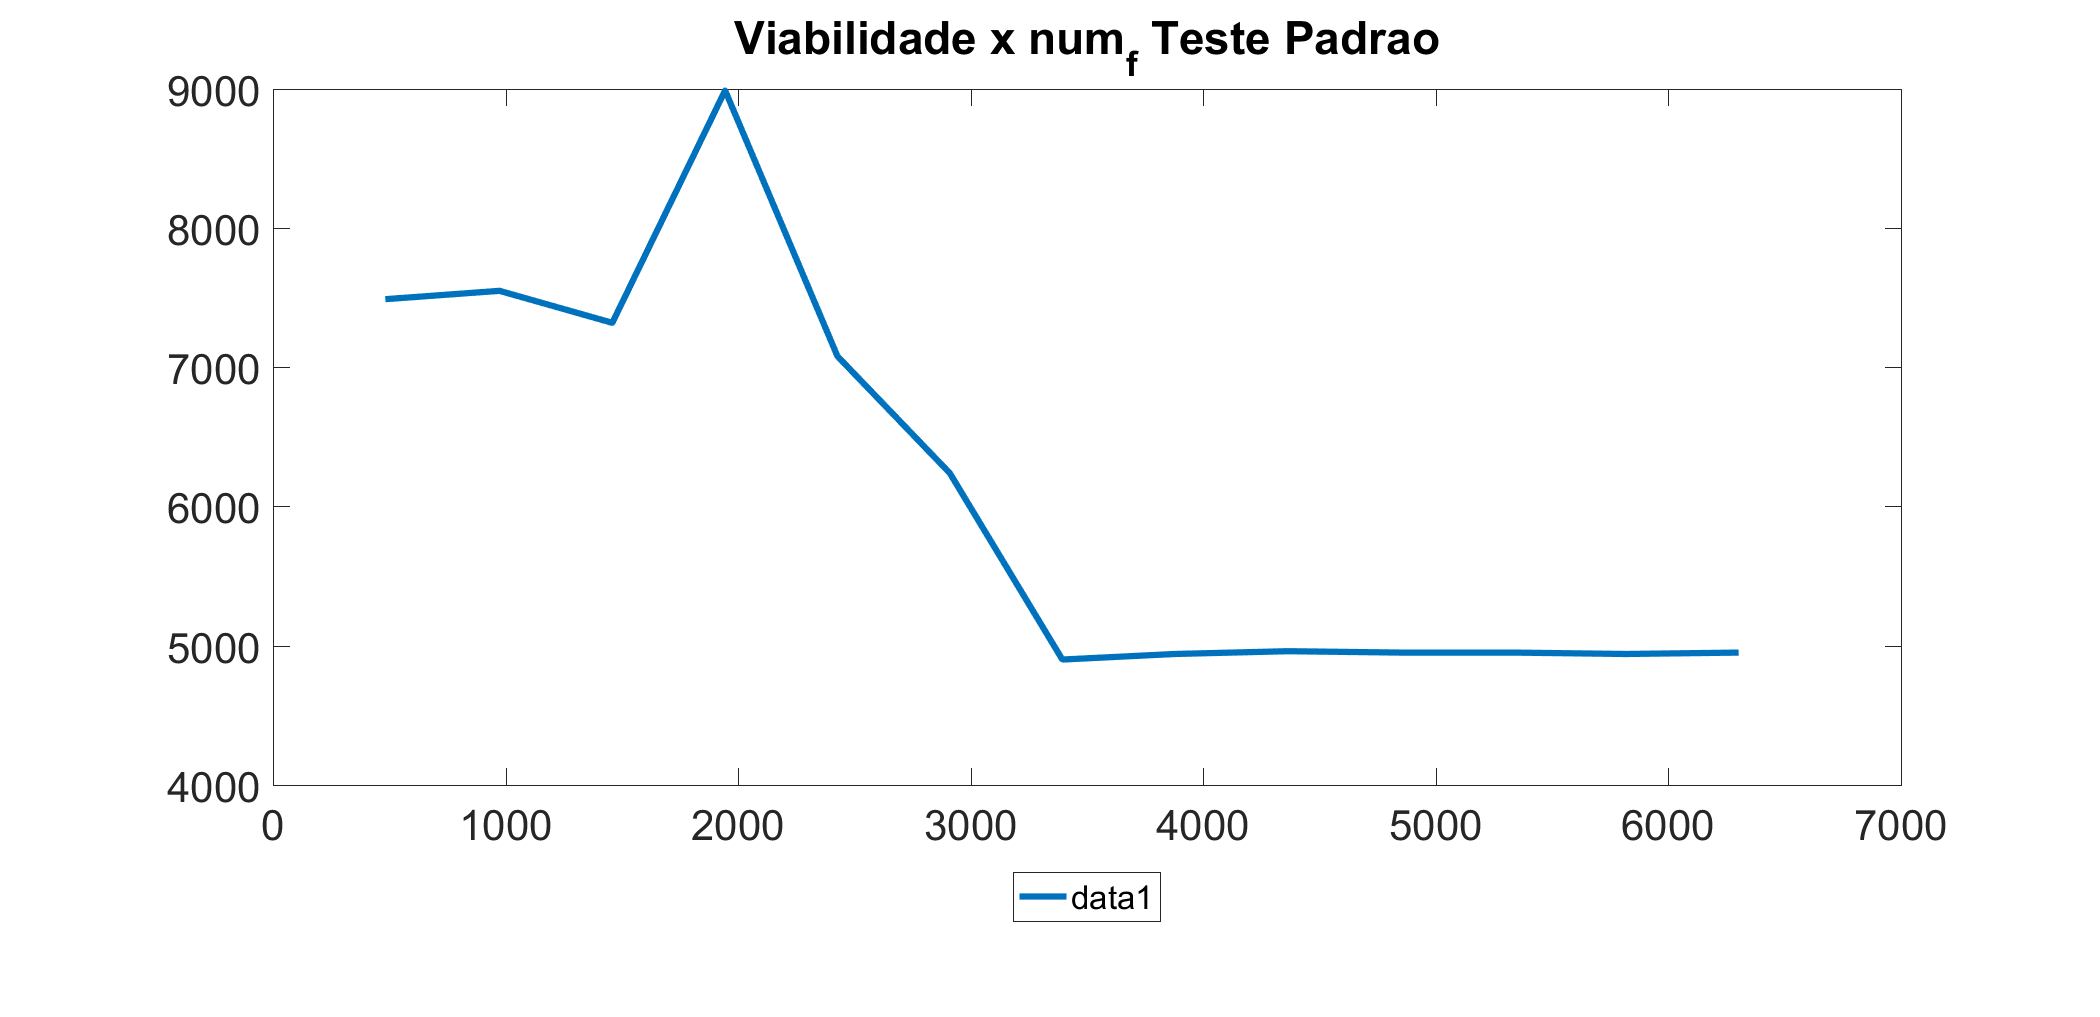
\includegraphics[scale=0.44]{Teste Padrao Viabilidade}
    \label{fig:t_padr_viab}
    \end{center}
\end{figure}

\subsection{Caso 1 - Variação da frequência}
Os resultados da variação da variavel de entrada frequência natural, que varia basicamente o comportamento da planta do
modelo dinâmico, exemplifica as diferenças nas amplitudes dos desvios entre a ponta e a referência e uma menor necessidade de compensação, assim como previsto
de um sistema de rigidez maior.
As diferenças podem ser observadas de forma clara se compadas as figuras \ref{fig:t_1a_vels}, \ref{fig:t_1b_vels} e \ref{fig:t_1c_vels},
comparando também as diferenças entre o comportamento do deslocamento e do caminho tomado entre os dois estremos do Caso (A e C) nas figuras
\ref{fig:t_1a_des}, \ref{fig:t_1c_des}, \ref{fig:t_1a_pos} e \ref{fig:t_1c_pos}.

\begin{figure}[H]
    \begin{center}
    \caption{Caso 1A - Comportamento no tempo das velocidades em x e y da ponta e da referência}
    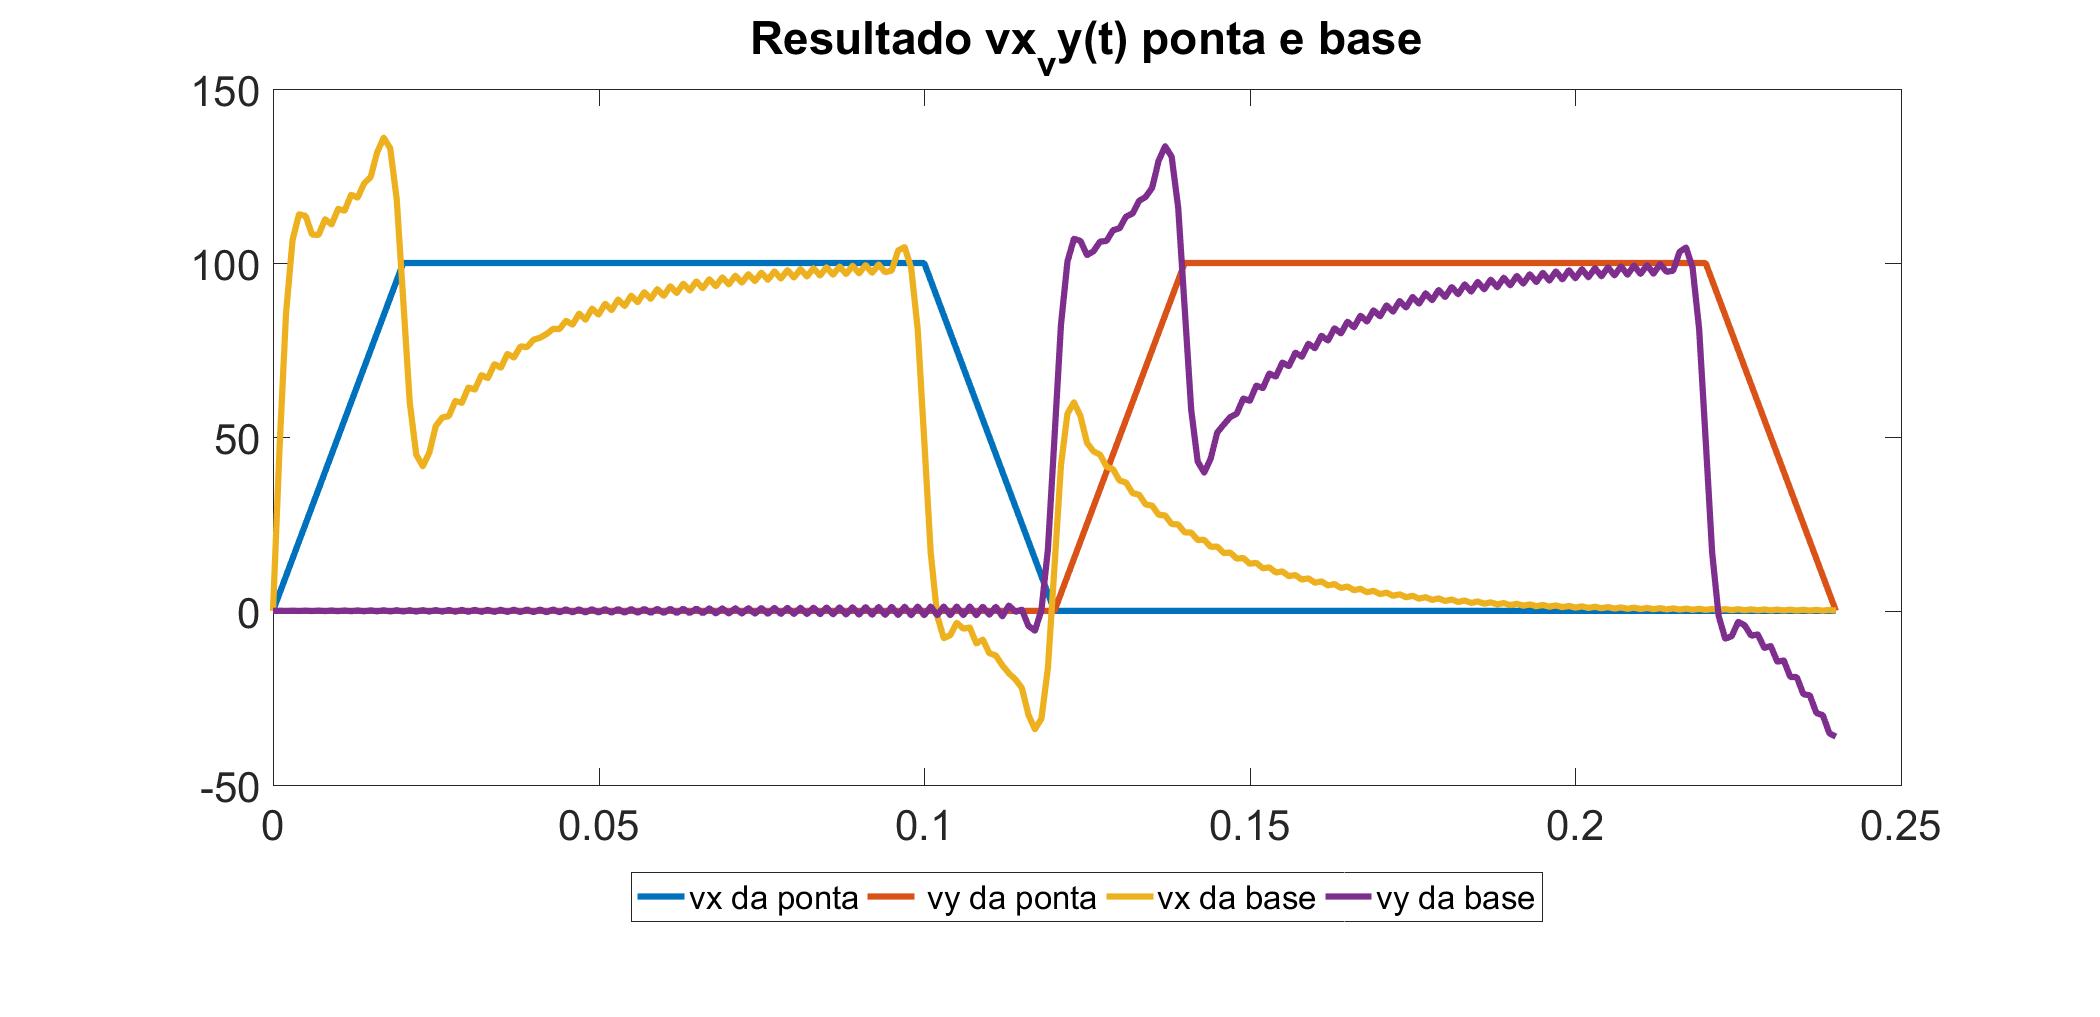
\includegraphics[scale=0.44]{Teste 1 A vels}
    \label{fig:t_1a_vels}
    \end{center}
\end{figure}

\begin{figure}[H]
    \begin{center}
    \caption{Caso 1B - Comportamento no tempo das velocidades em x e y da ponta e da referência}
    \label{fig:t_1b_vels}
    \end{center}
\end{figure}

\begin{figure}[H]
    \begin{center}
    \caption{Caso 1C - Comportamento no tempo das velocidades em x e y da ponta e da referência}
    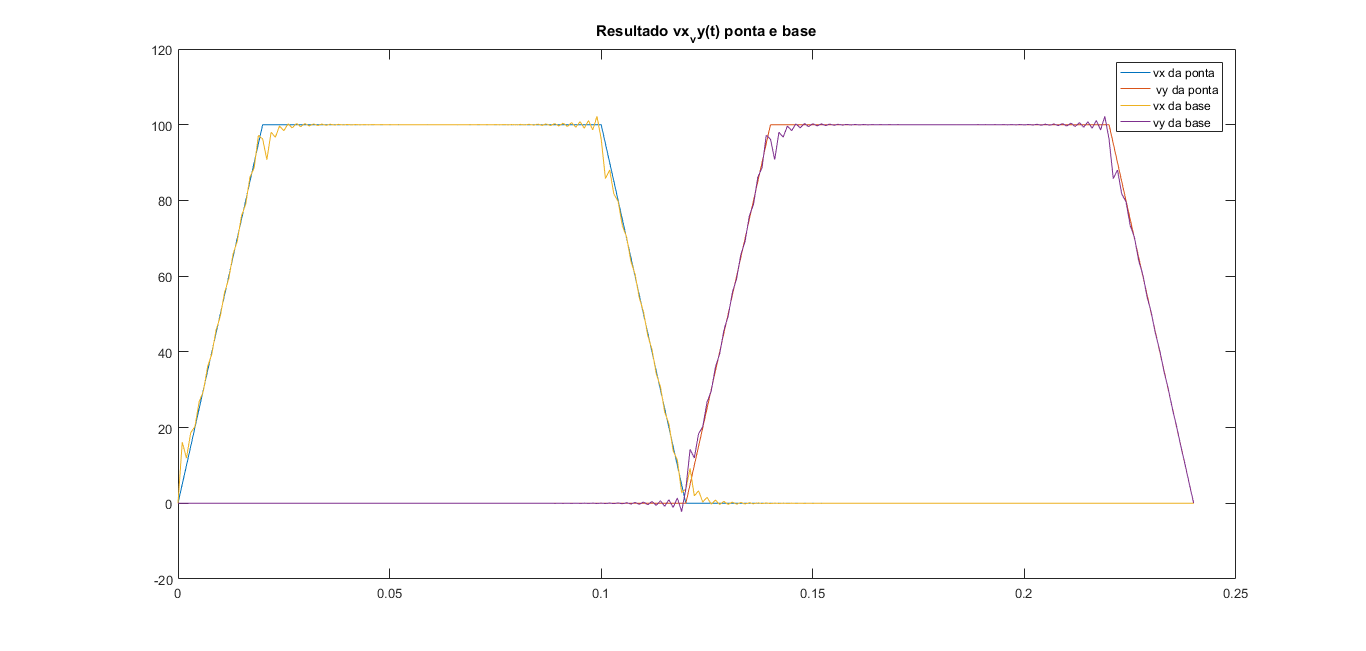
\includegraphics[scale=0.44]{Teste 1 C vels}
    \label{fig:t_1c_vels}
    \end{center}
\end{figure}

\begin{figure}[H]
    \begin{center}
    \caption{Caso 1A - Comportamento no tempo dos deslocamentos em x e y da ponta e da referência}
    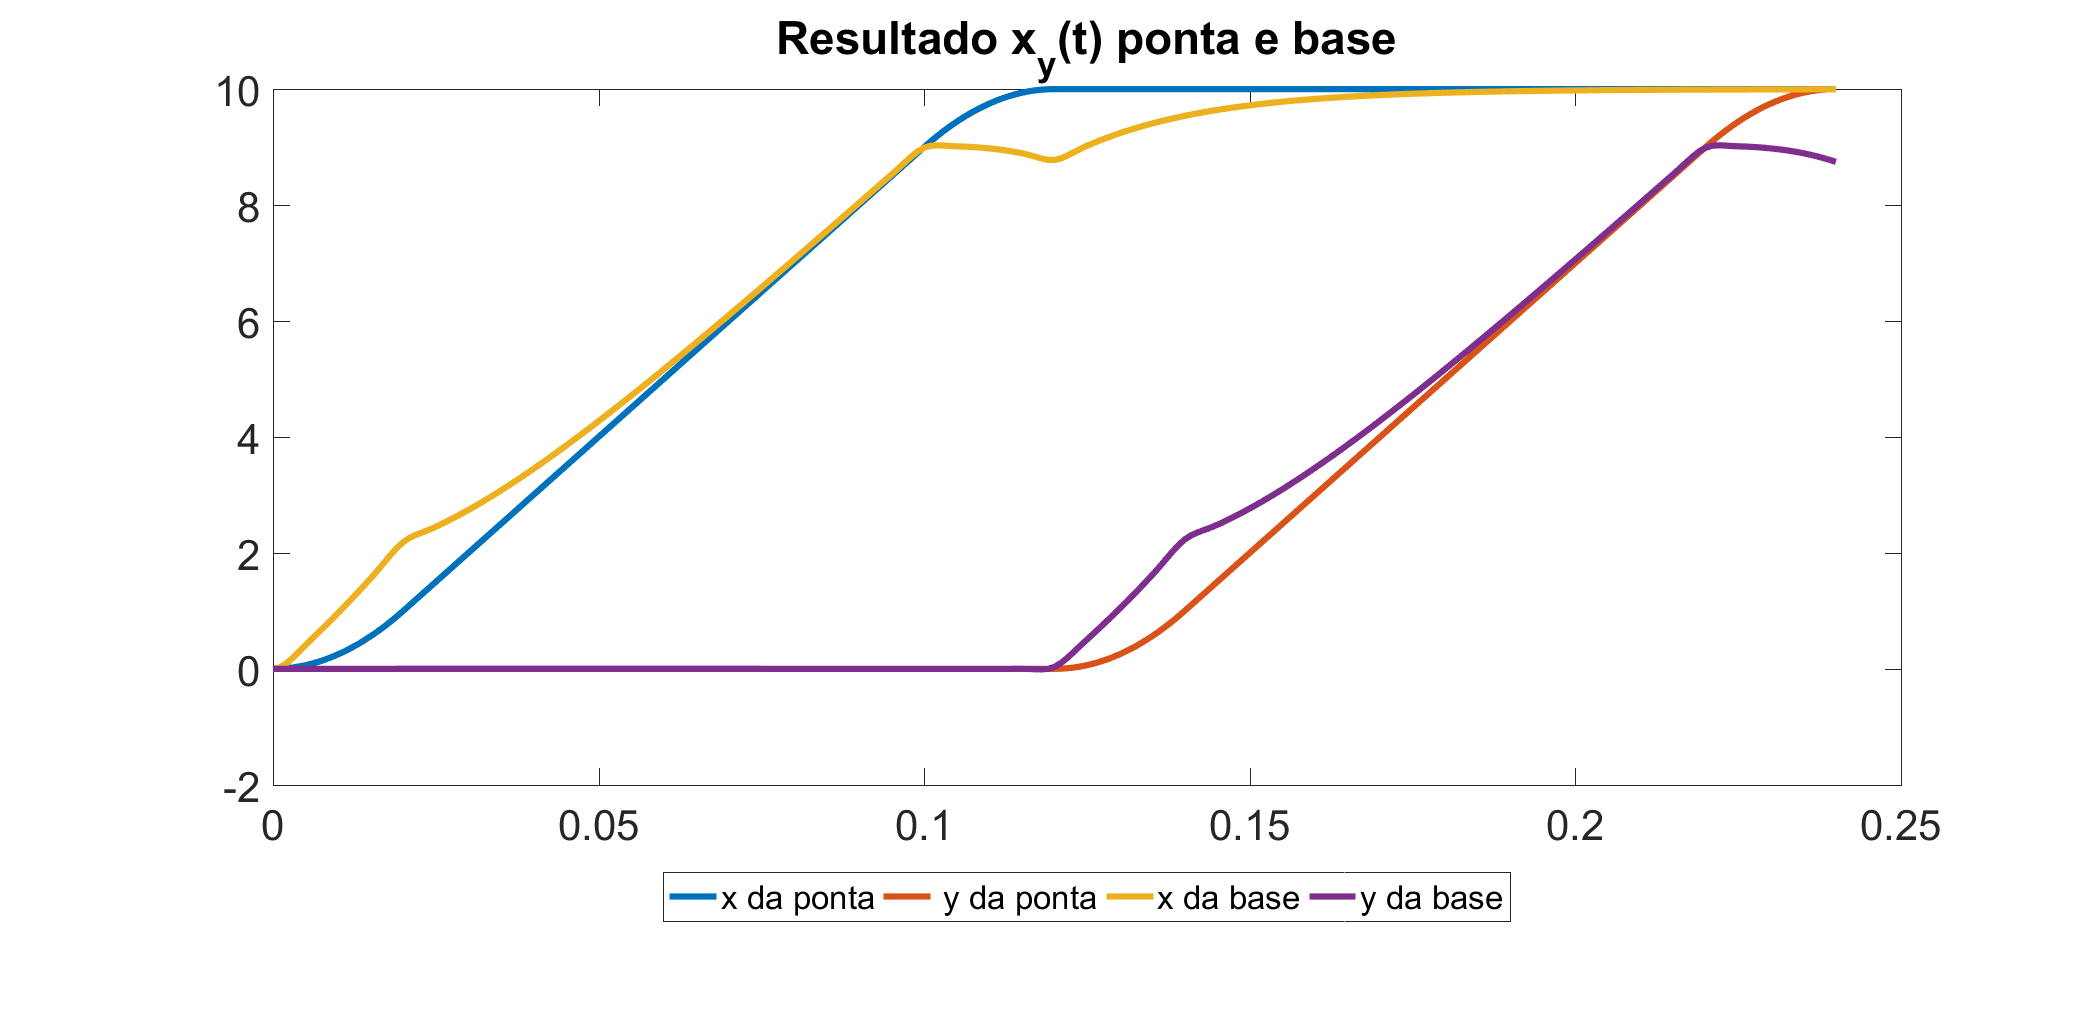
\includegraphics[scale=0.44]{Teste 1 A des}
    \label{fig:t_1a_des}
    \end{center}
\end{figure}

\begin{figure}[H]
    \begin{center}
    \caption{Caso 1C - Comportamento no tempo dos deslocamentos em x e y da ponta e da referência}
    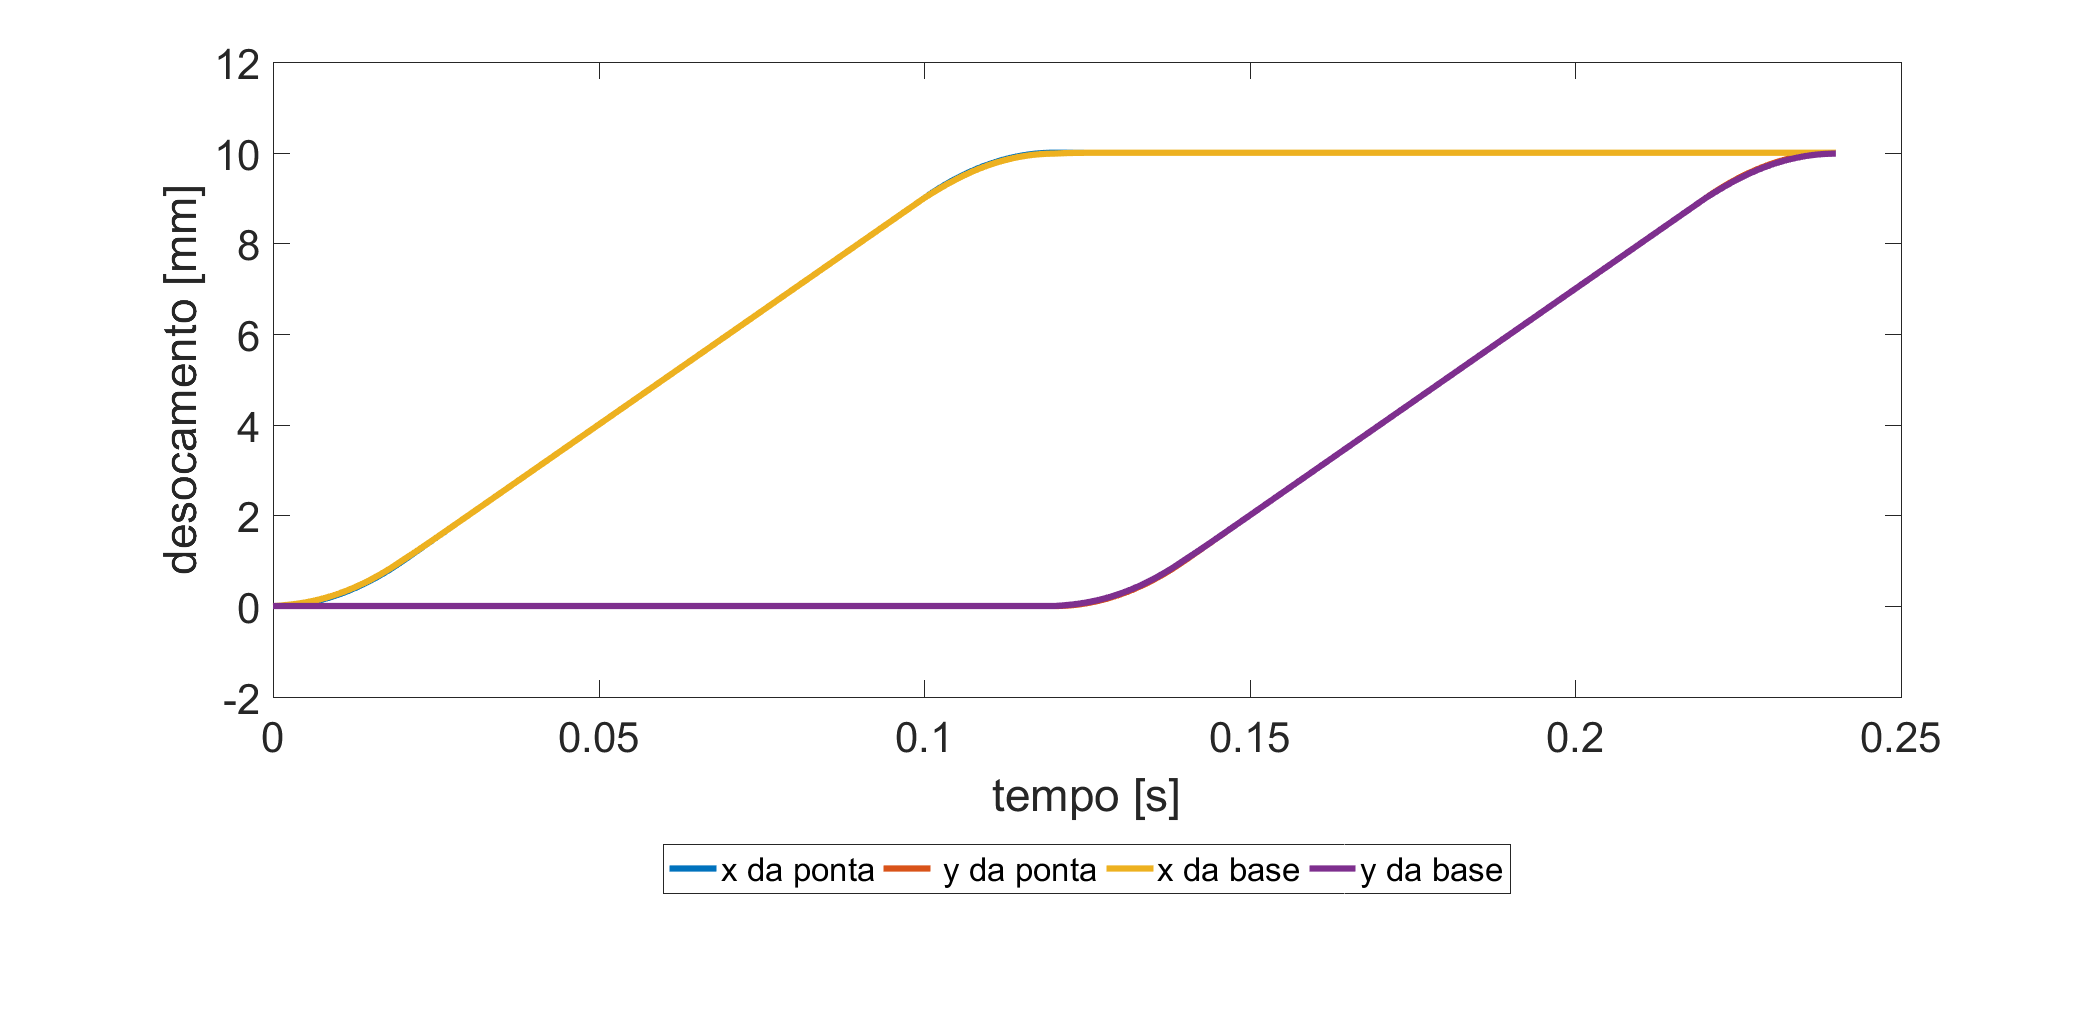
\includegraphics[scale=0.44]{Teste 1 C des}
    \label{fig:t_1c_des}
    \end{center}
\end{figure}

\begin{figure}[H]
    \begin{center}
    \caption{Caso 1A - Caminho percorrido x vs y da ponta e da referência}
    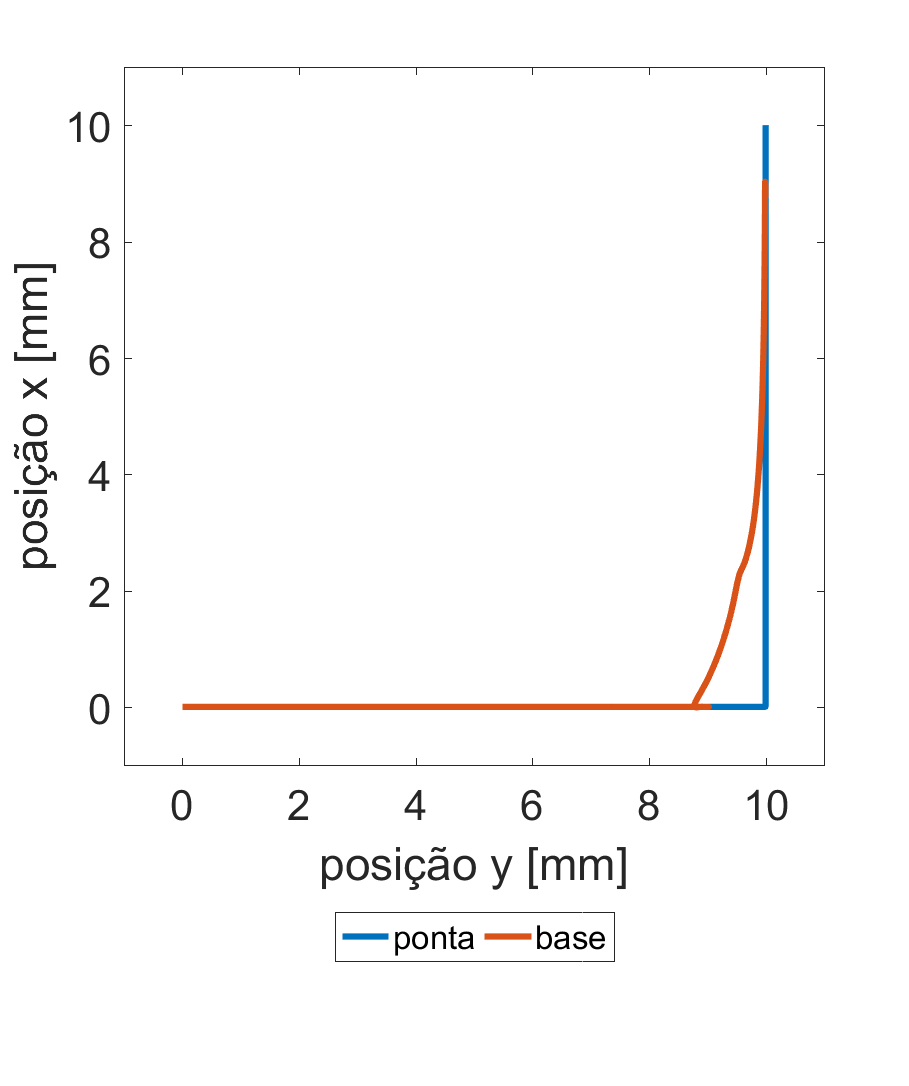
\includegraphics[scale=0.44]{Teste 1 A pos}
    \label{fig:t_1a_pos}
    \end{center}
\end{figure}

\begin{figure}[H]
    \begin{center}
    \caption{Caso 1C - Caminho percorrido x vs y da ponta e da referência}
    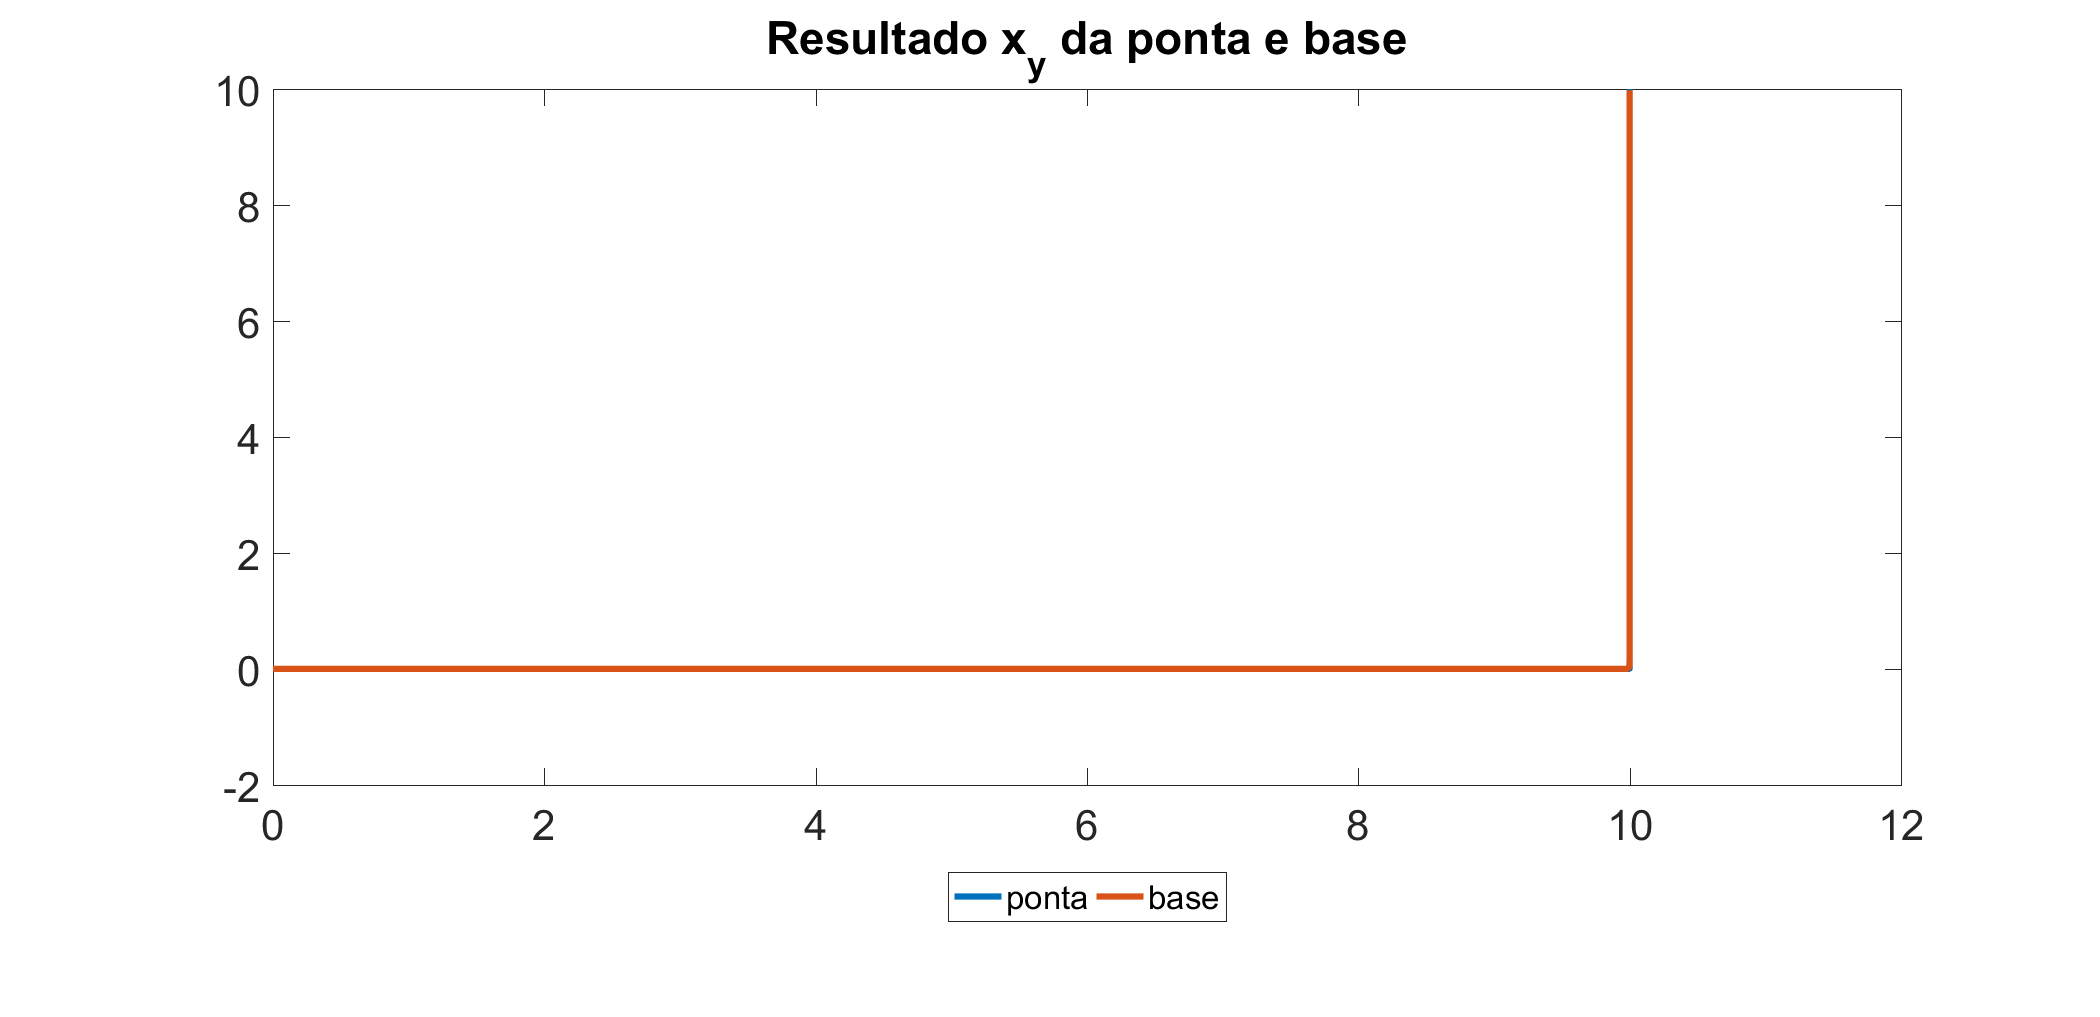
\includegraphics[scale=0.44]{Teste 1 C pos}
    \label{fig:t_1c_pos}
    \end{center}
\end{figure}

Já na figura \ref{fig:t_1_viab} é possivel notar um comportamento semelhante de convergência, mas nota-se que
nos Casos de maior rigidez a viabilidade alcançada foi menor, ou seja, menores vioções das restrições impostas, dados
primordialmente pelos menores desvios e menor necessidade de compensação.
Essa característica pode ser observada também nos tempos de simulação que foram reduzindo de $96,76 s$ (Caso A) até
$80,77 s$ (Caso C), com o Caso B ficando entre os dois com $89,04 s$, todos esses com vetores de posição de 241 elementos.

\begin{figure}[H]
    \begin{center}
    \caption{Caso 1 - Num de fun x Viabilidade}
    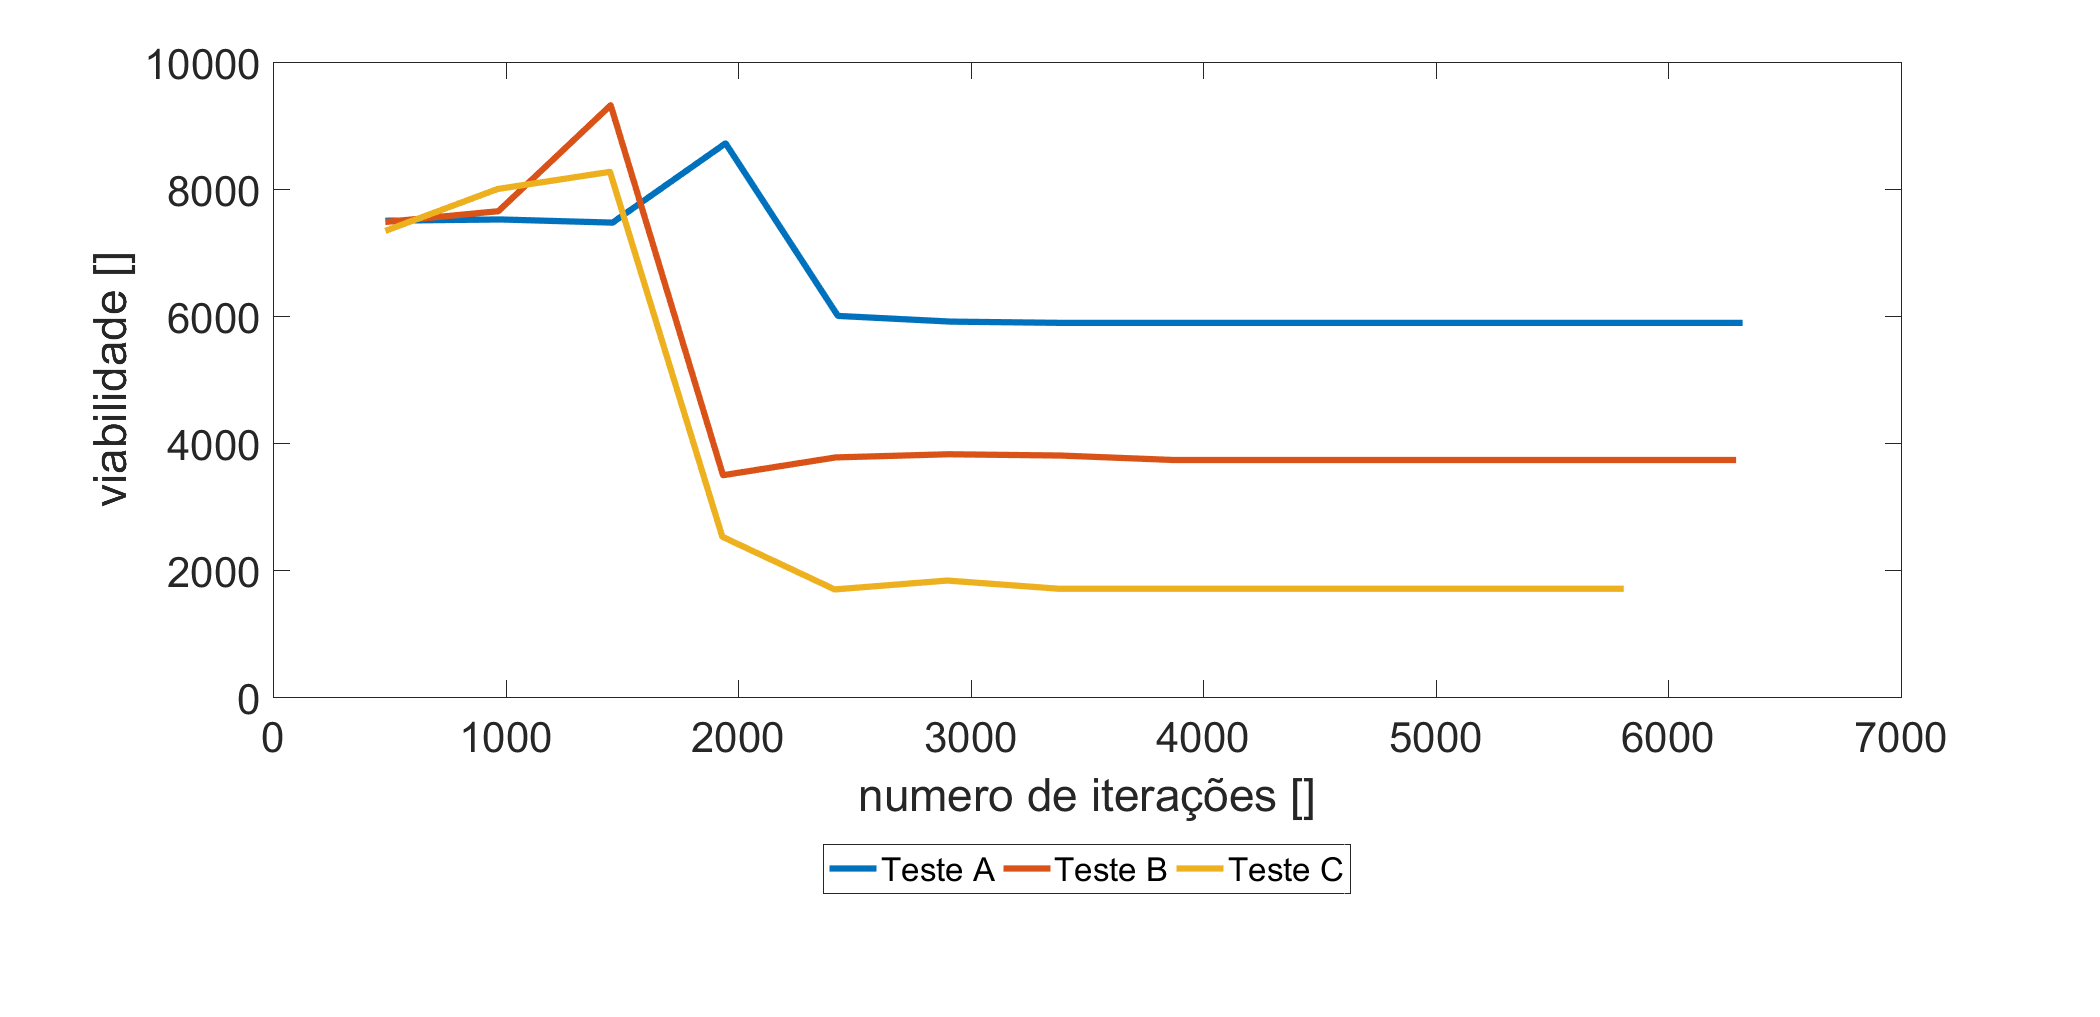
\includegraphics[scale=0.44]{Teste 1 Viabilidade}
    \label{fig:t_1_viab}
    \end{center}
\end{figure}

\subsection{Caso 2 - Variação do coeficiente de amortecimento}
No Caso 2, que varia o coeficiente de amortecimento, podemos avaliar de forma mais clara as diferenças através das figuras
\ref{fig:t_2b_pos} e \ref{fig:t_2c_pos} que mostram as curvas dos caminhos do Caso b e c respectivamente, podemos comparar também
com a figura \ref{fig:t_padr_pos} que possui um coeficiente intermediario entre os Casos A e B.
Sendo o Caso A não apresentado, por não ter convergido, apresentando praticamente o mesmos valores de entrada, esse comportamento
é identificado na figura \ref{fig:t_2_viab}, onde podemos observar também um padrão convergência para valores de viabilidade menor conforme
coeficiente de amortecimento também aumenta, ou seja, uma maior facilidade de compensar os desvios.
Todos se mantiveram com 241 elementos nos vetores de posição e tempos de simulação de $69, 89 e 52 s$ para os Casos 2A, 2B e 2C respectivamente.

\begin{figure}[H]
    \begin{center}
    \caption{Caso 2B - Caminho percorrido x vs y da ponta e da referência}
    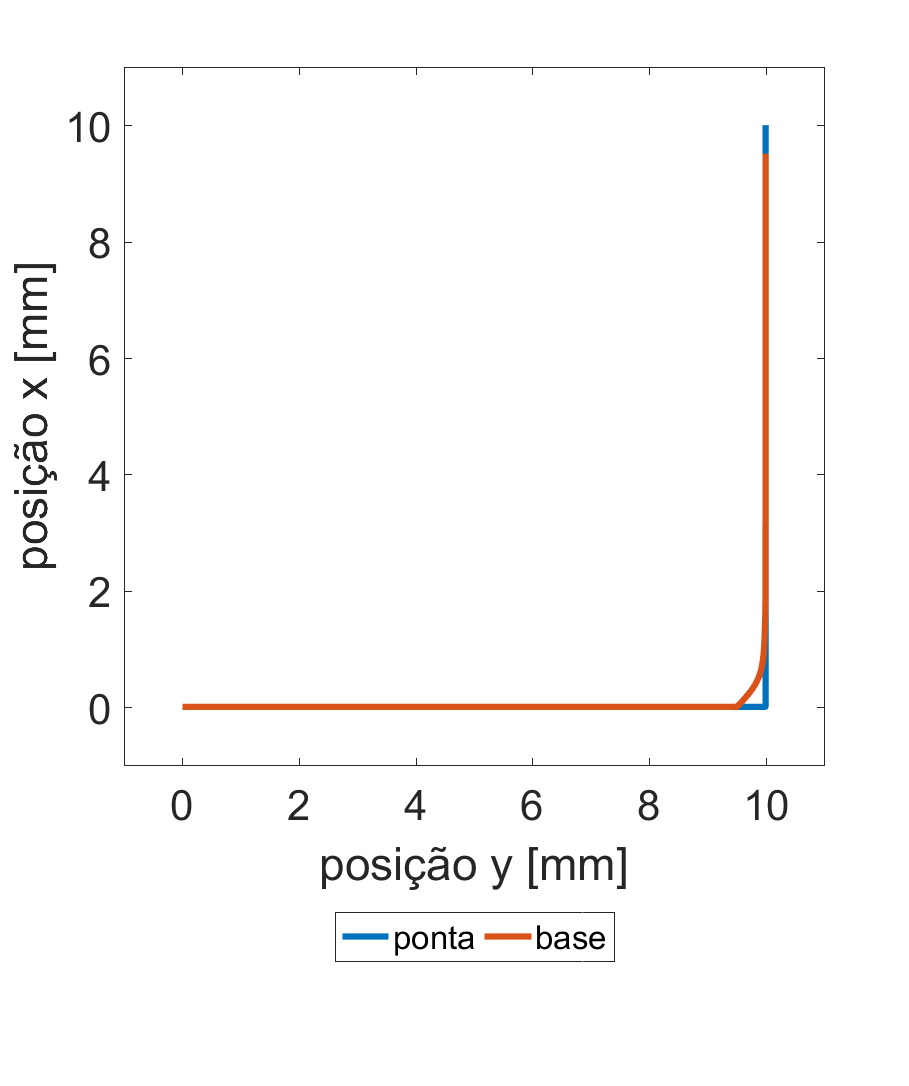
\includegraphics[scale=0.44]{Teste 2 B pos}
    \label{fig:t_2b_pos}
    \end{center}
\end{figure}

\begin{figure}[H]
    \begin{center}
    \caption{Caso 2C - Caminho percorrido x vs y da ponta e da referência}
    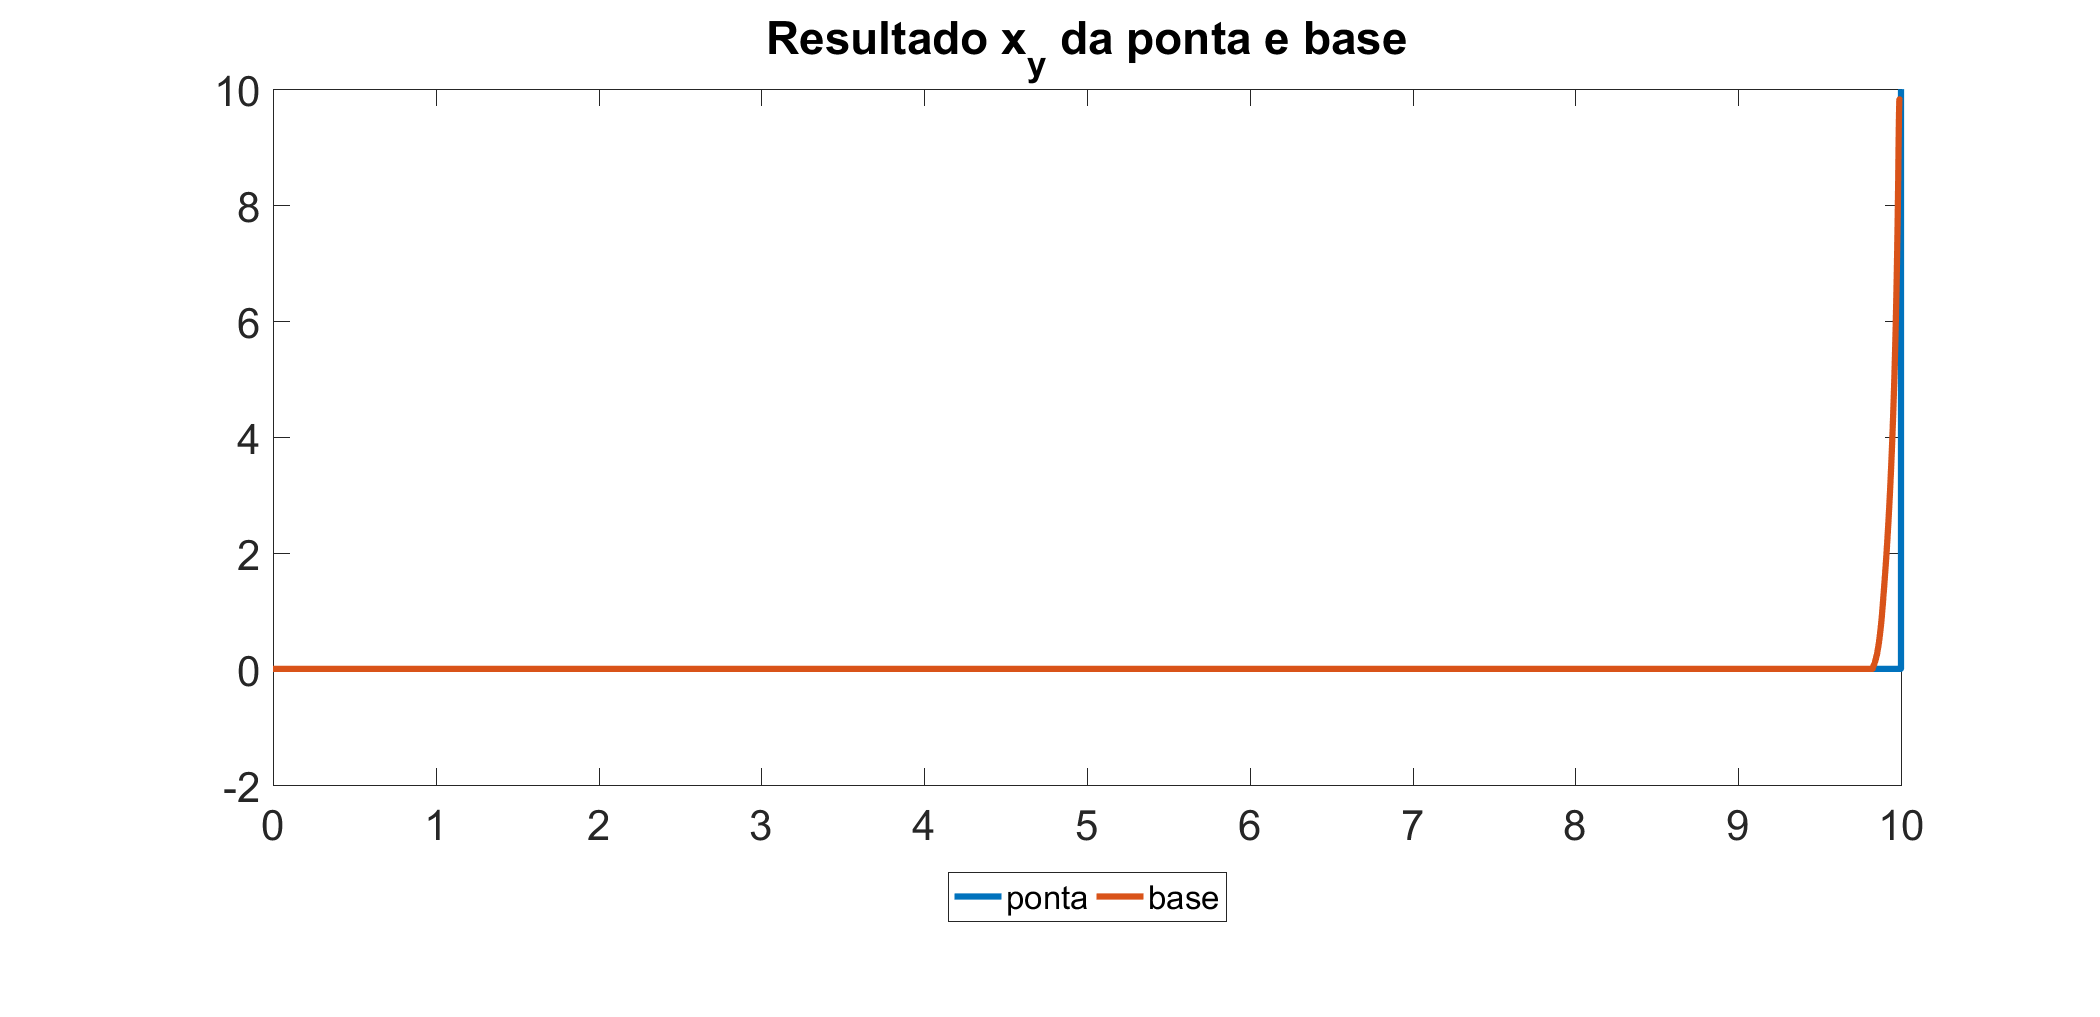
\includegraphics[scale=0.44]{Teste 2 C pos}
    \label{fig:t_2c_pos}
    \end{center}
\end{figure}

\begin{figure}[H]
    \begin{center}
    \caption{Caso 2 - Num de fun x Viabilidade}
    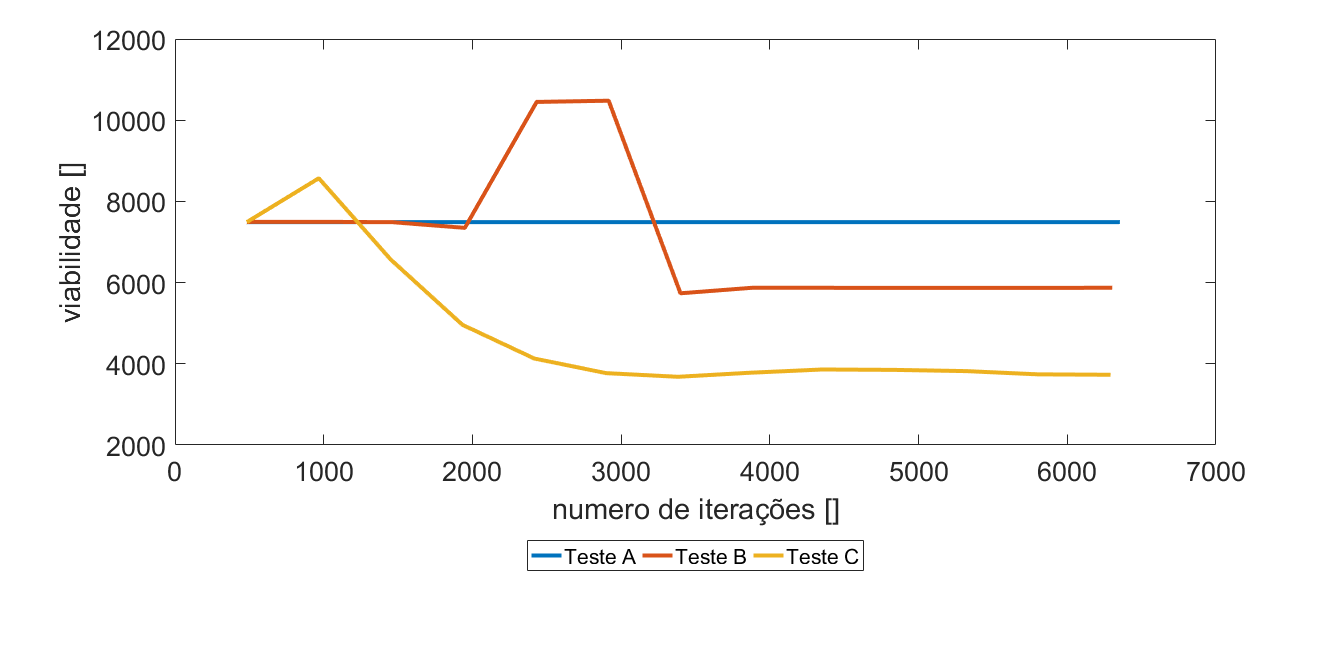
\includegraphics[scale=0.44]{Teste 2 Viabilidade}
    \label{fig:t_2_viab}
    \end{center}
\end{figure}

\subsection{Caso 3 - Variação na aceleração}
Podemos observar na figura \ref{fig:t_3a_vels} uma curva de velocidade diferente, dado que reduzimos a aceleração
na geração de comando, a velocidade não conseguiu alcançar o nível de velocidade desejada e assim toma-se a forma de um triangulo.
Já pela figura \ref{fig:t_3_viab}, podemos observar que a função teve dificuldades para solucionar o Caso A, enquanto para o Caso B
teve um comportamento semelhante aos Casos anteriores, com um aumento nos valores de viabilidade.
Um dos motivos possíveis para essa dificuldade se da no tamanho dos vetores trabalhados, no Caso A o vetor de posições
possuía 401 elementos, e levou $195 s$ para realizar a simulação, enquanto para o Caso B o vetor de posição possuia 221 elementos
e levou $78 s$, valores bem mais próximos aos Casos referência assim como suas curvas.

\begin{figure}[H]
    \begin{center}
    \caption{Caso 3A - Comportamento no tempo das velocidades em x e y da ponta e da referência}
    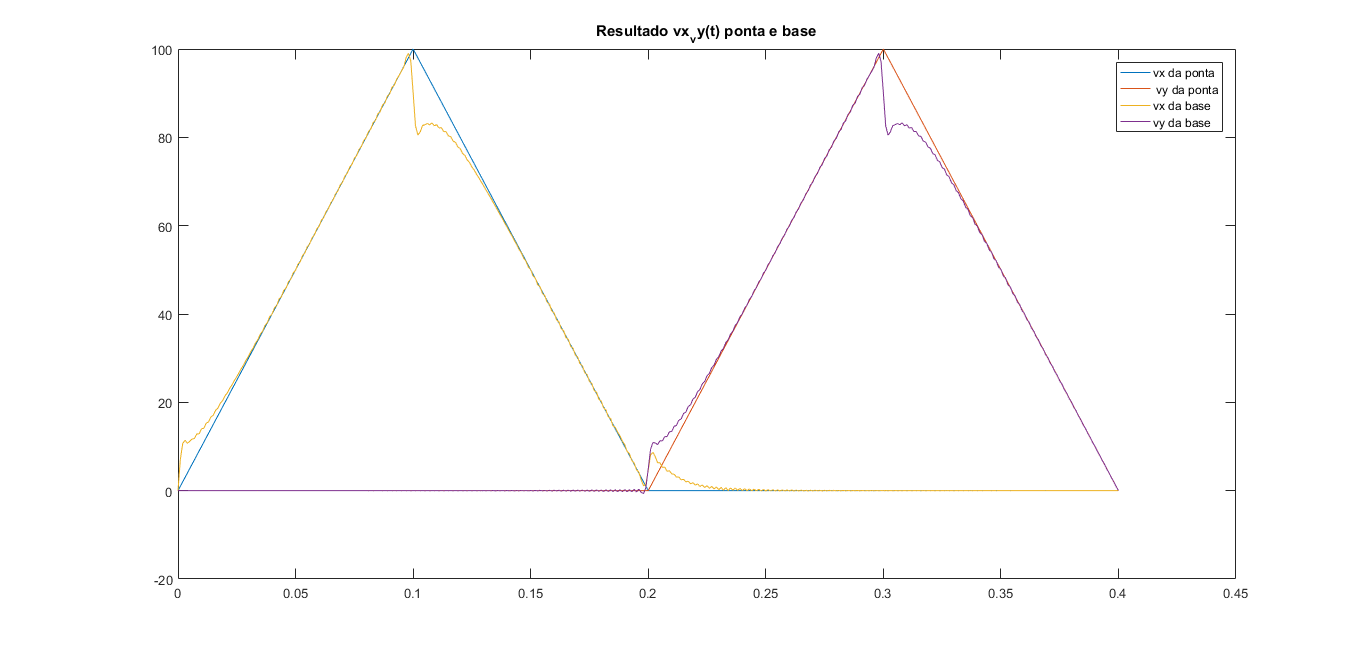
\includegraphics[scale=0.44]{Teste 3 A vels}
    \label{fig:t_3a_vels}
    \end{center}
\end{figure}

\begin{figure}[H]
    \begin{center}
    \caption{Caso 3 - Num de fun x Viabilidade}
    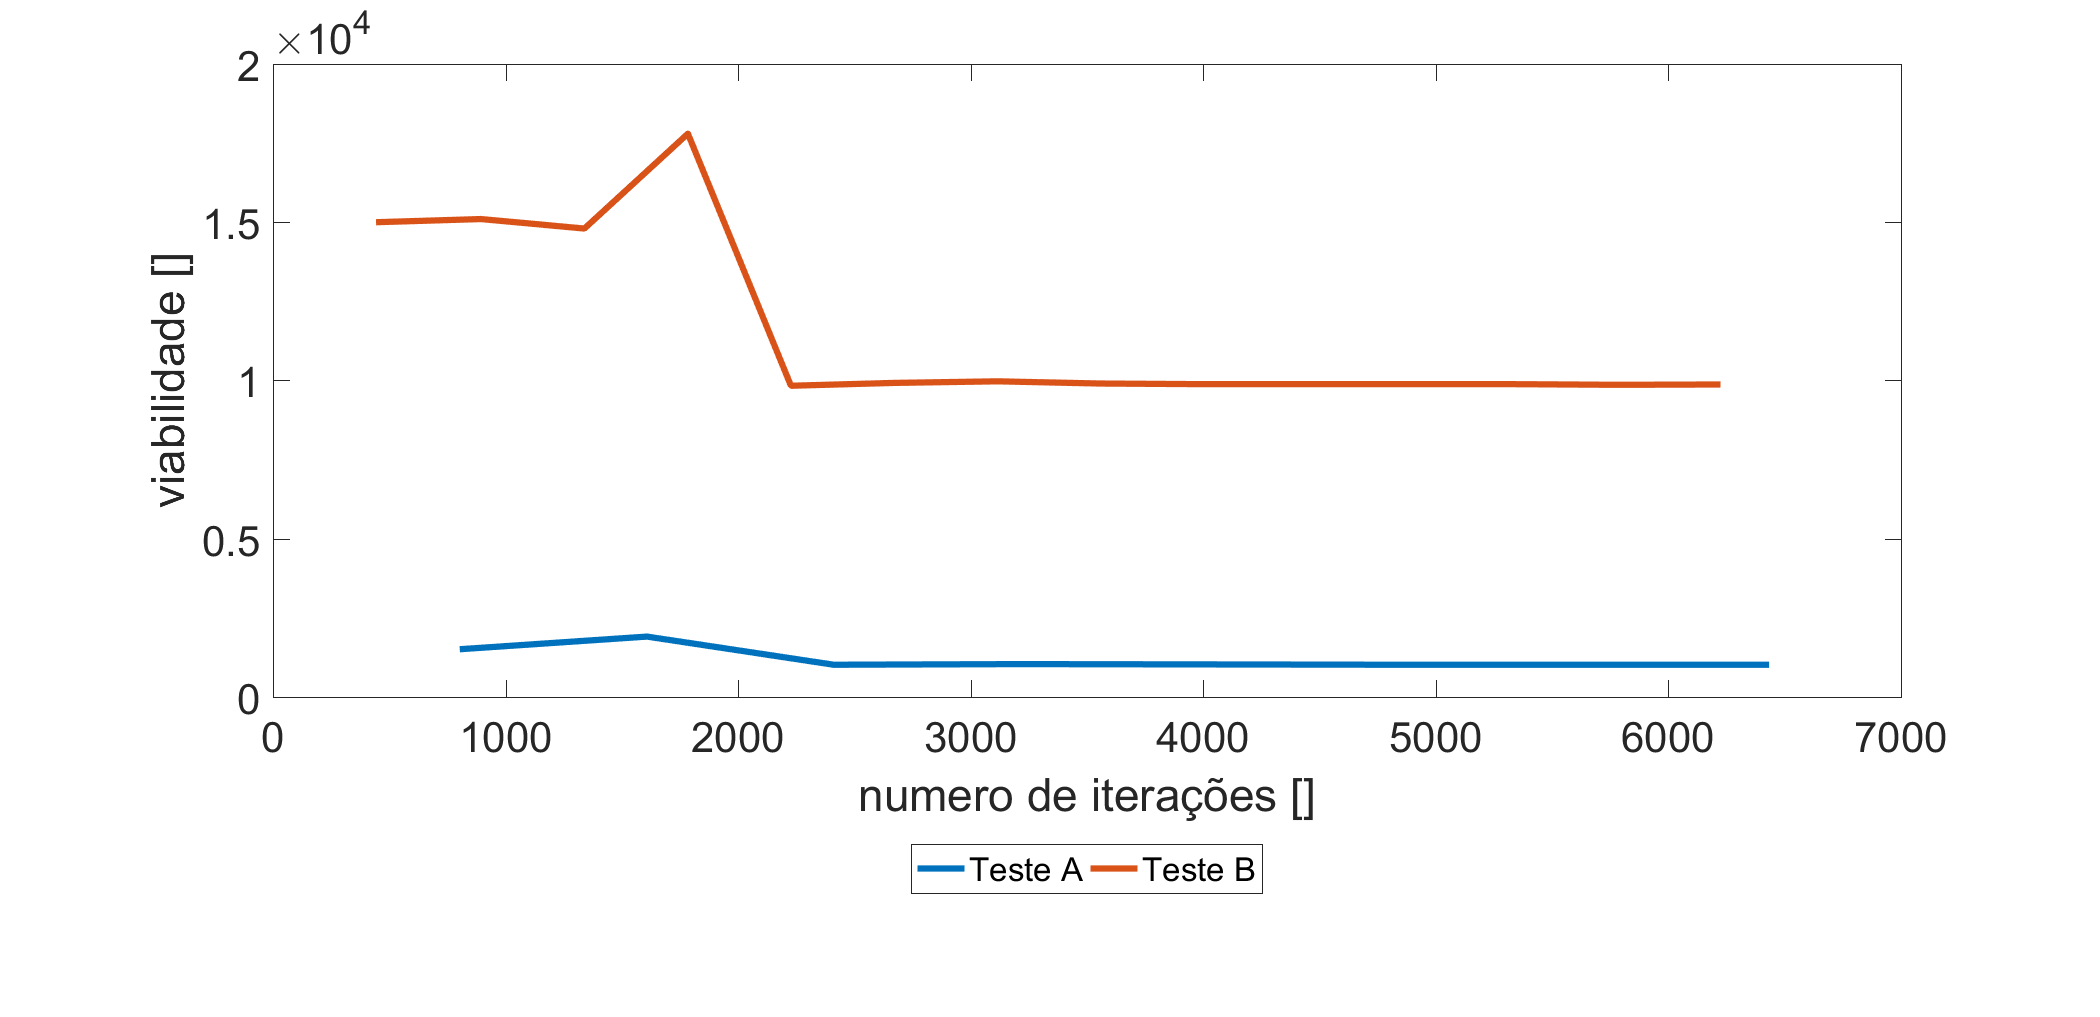
\includegraphics[scale=0.44]{Teste 3 Viabilidade}
    \label{fig:t_3_viab}
    \end{center}
\end{figure}

\subsection{Caso 4 - Variação da velocidade}
Variando a velocidade desejada, através do Gcode de entrada, analisamos os impactos de velocidades desajadas mais baixas e mais altas.
As mais baixas (Caso A) tem seu maior impacto no tamanho dos vetores e no tempo de simulção, já que percorre o percurso em mais tempo,
gerando uma malha com mais pontos, dada a resolução de $dt$ como fixa. Ficando assim com um tempo de simulação de $219 s$ e 421 elementos nos vetores de posição.
Enquanto para o Caso B, o tempo de simulação ficou em $60 s$ e com 181 elementos, mas dada a velocidade desejada maior e uma mesma aceleração máxima
na geração de comando, a curva de velocidade se assemelha a do Caso 3A exposta na figura \ref{fig:t_4b_vels} e com a curva de deslocamentos apresentada na figura \ref{fig:t_4b_des}.
Podemos comparar também o padrão de convergência na figura \ref{fig:t_4_viab}

\begin{figure}[H]
    \begin{center}
    \caption{Caso 4B - Comportamento no tempo das velocidades em x e y da ponta e da referência}
    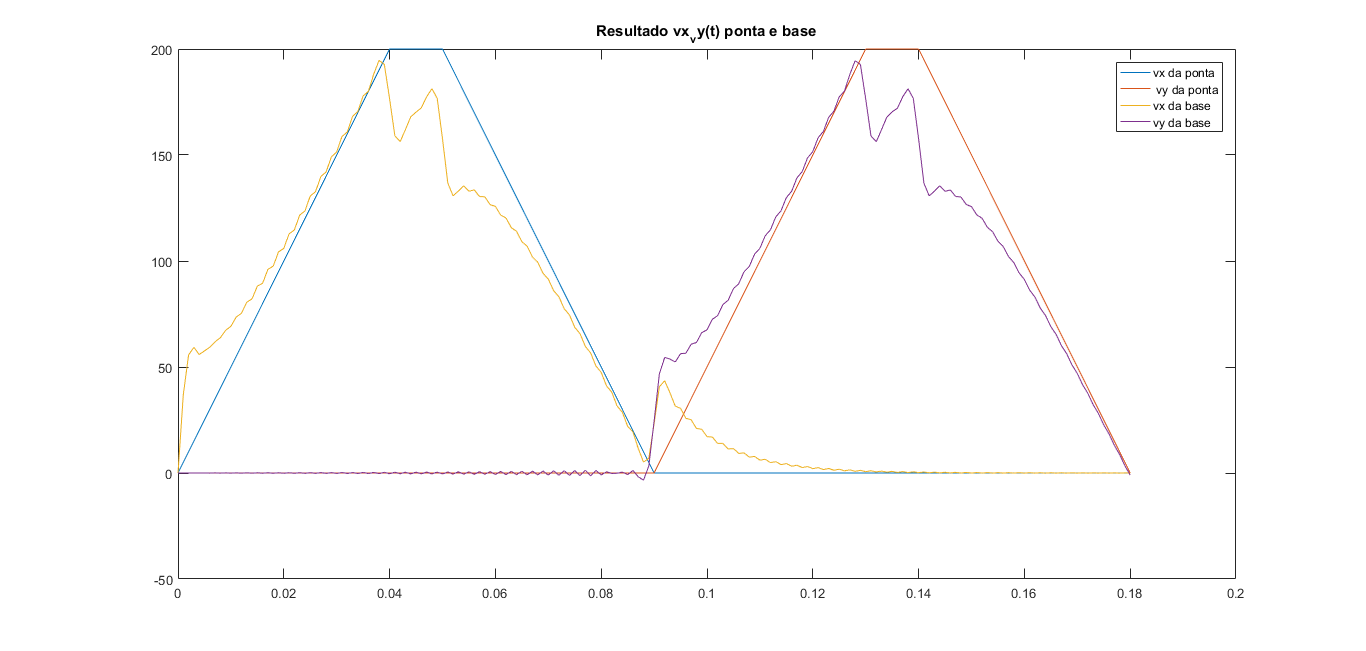
\includegraphics[scale=0.44]{Teste 4 B vels}
    \label{fig:t_4b_vels}
    \end{center}
\end{figure}

\begin{figure}[H]
    \begin{center}
    \caption{Caso 4B - Comportamento no tempo dos deslocamentos em x e y da ponta e da referência}
    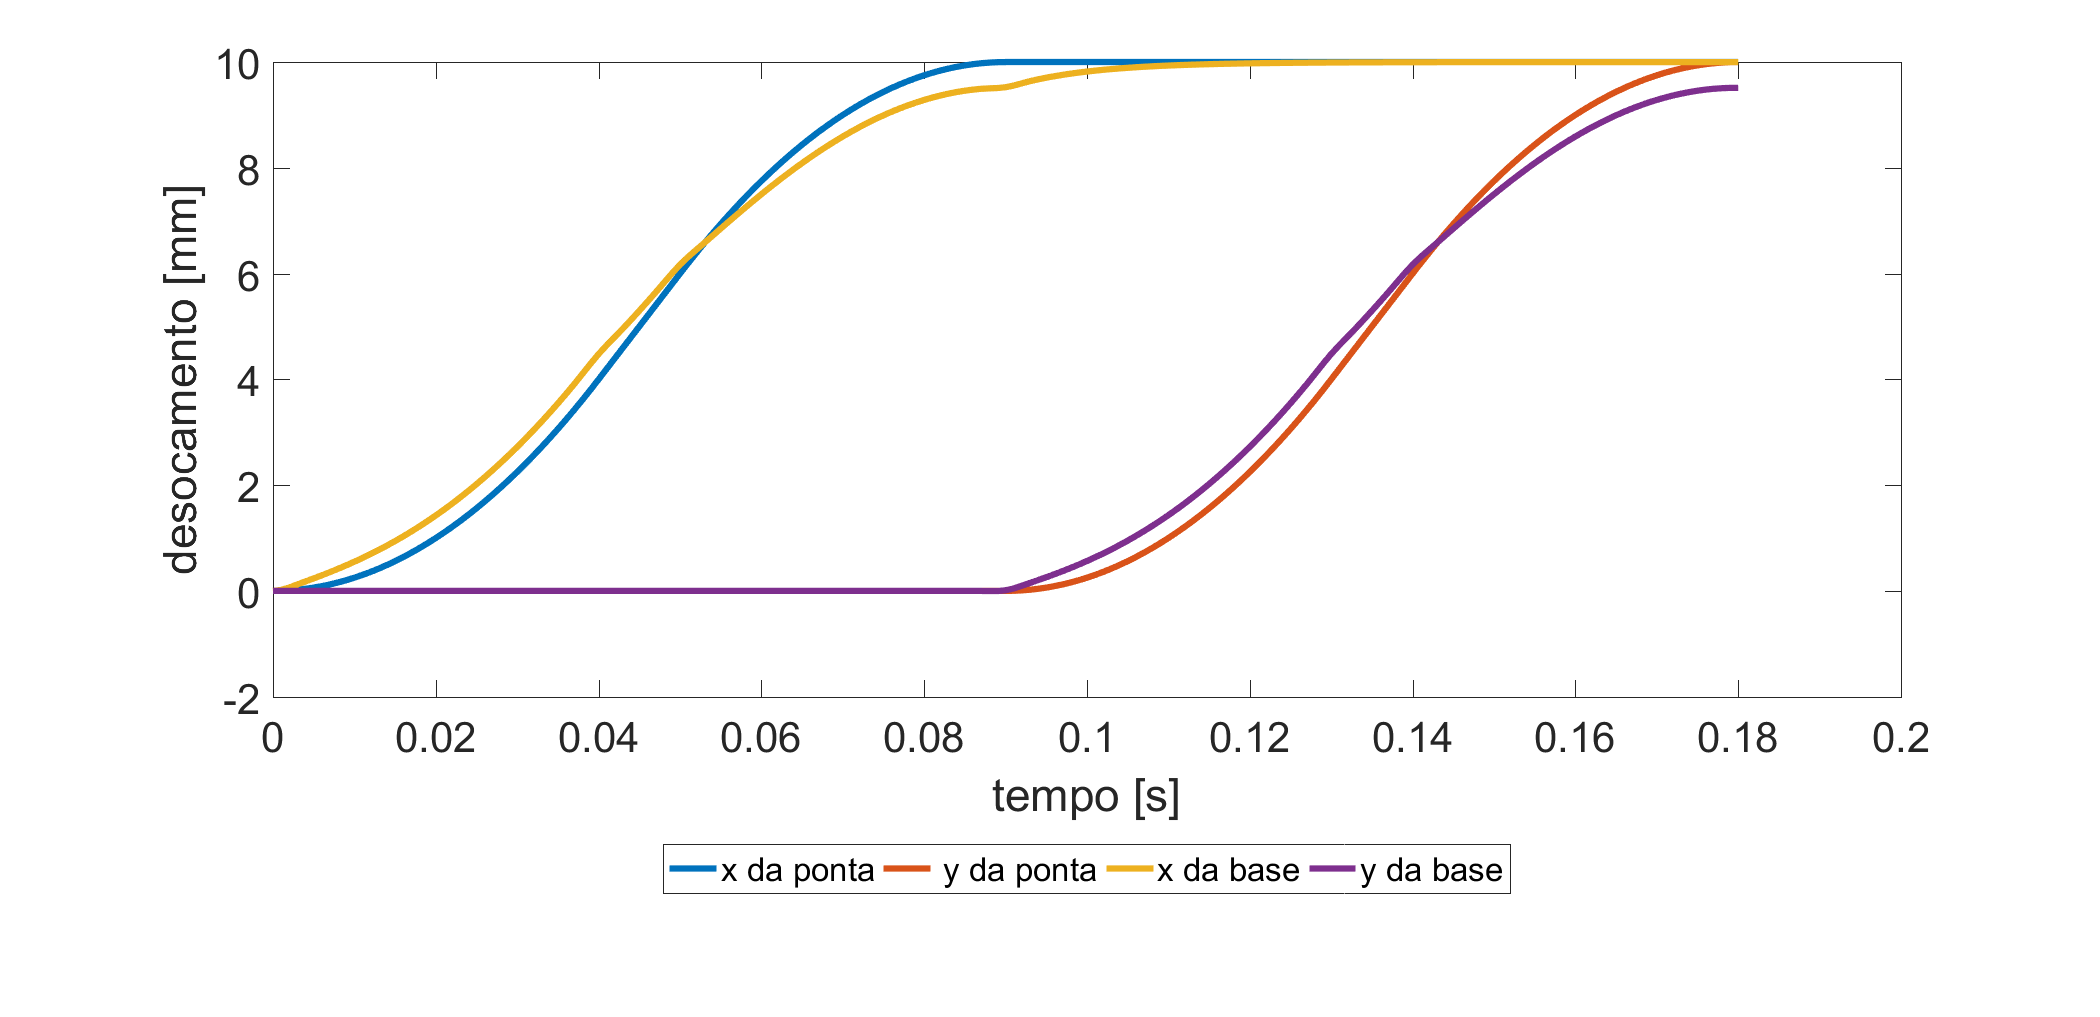
\includegraphics[scale=0.44]{Teste 4 B des}
    \label{fig:t_4b_des}
    \end{center}
\end{figure}

\begin{figure}[H]
    \begin{center}
    \caption{Caso 4 - Num de fun x Viabilidade}
    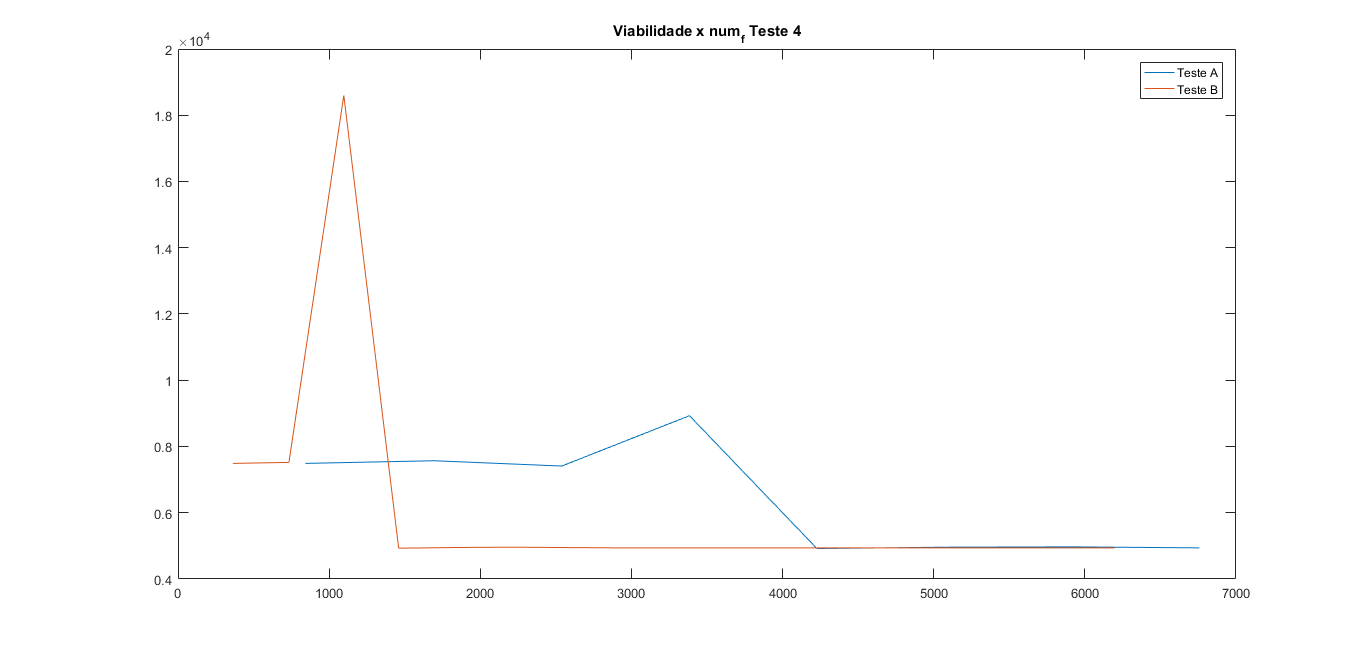
\includegraphics[scale=0.44]{Teste 4 Viabilidade}
    \label{fig:t_4_viab}
    \end{center}
\end{figure}

\subsection{Caso 5 - Variação do passo de tempo}
Por fim, evidenciamos as diferenças nos resultados com resoluções diferentes para a malha de tempo e seu impacto nas respostas.
As figuras \ref{fig:t_5a_vels}, \ref{fig:t_5b_vels} e \ref{fig:t_5c_vels} revelam principalmente a influência desse parâmetro
nas oscilações nos gráficos de velocidade, entretanto a diferença é menos nítida se avaliados os gráficos de deslocamento das figuras
\ref{fig:t_5a_des}, \ref{fig:t_5b_des} e \ref{fig:t_5c_des}.

\begin{figure}[H]
    \begin{center}
    \caption{Caso 5A - Comportamento no tempo das velocidades em x e y da ponta e da referência}
    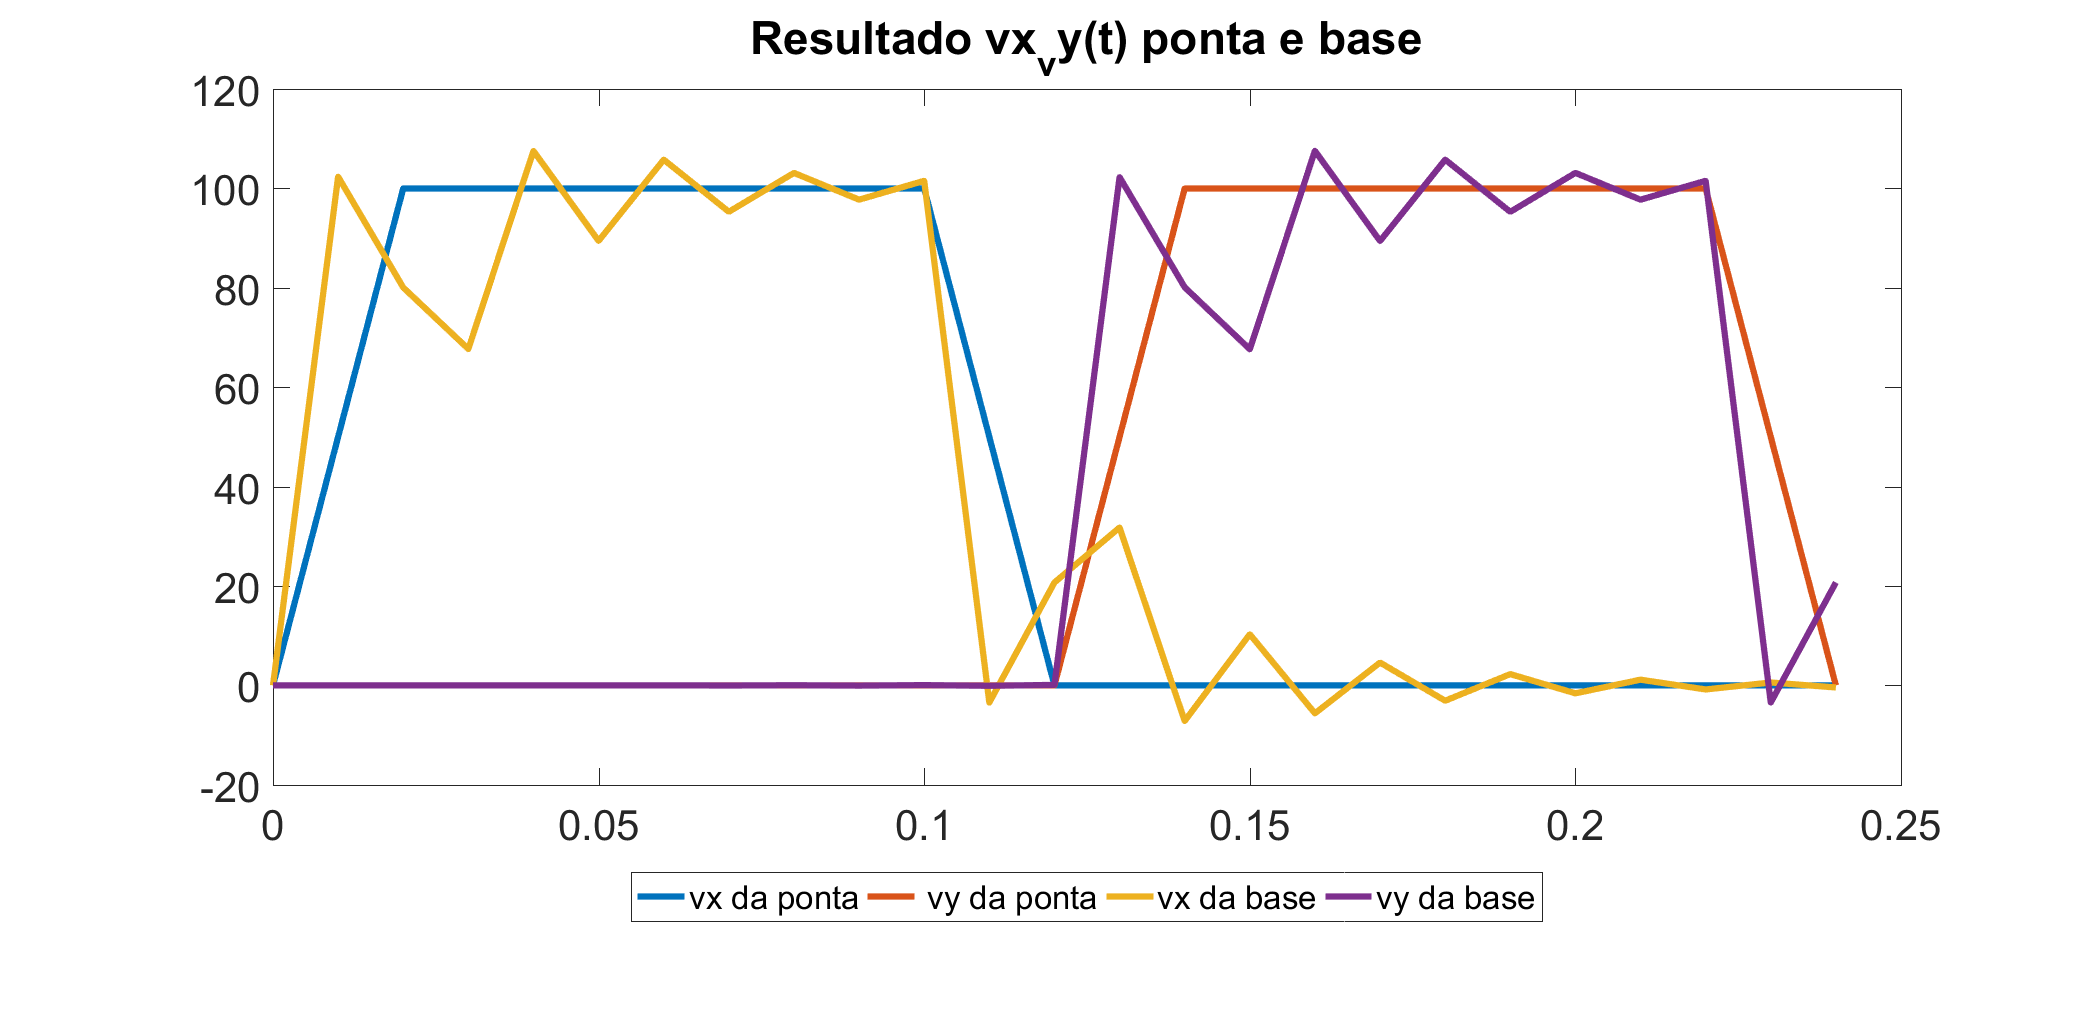
\includegraphics[scale=0.44]{Teste 5 A vels}
    \label{fig:t_5a_vels}
    \end{center}
\end{figure}

\begin{figure}[H]
    \begin{center}
    \caption{Caso 5B - Comportamento no tempo das velocidades em x e y da ponta e da referência}
    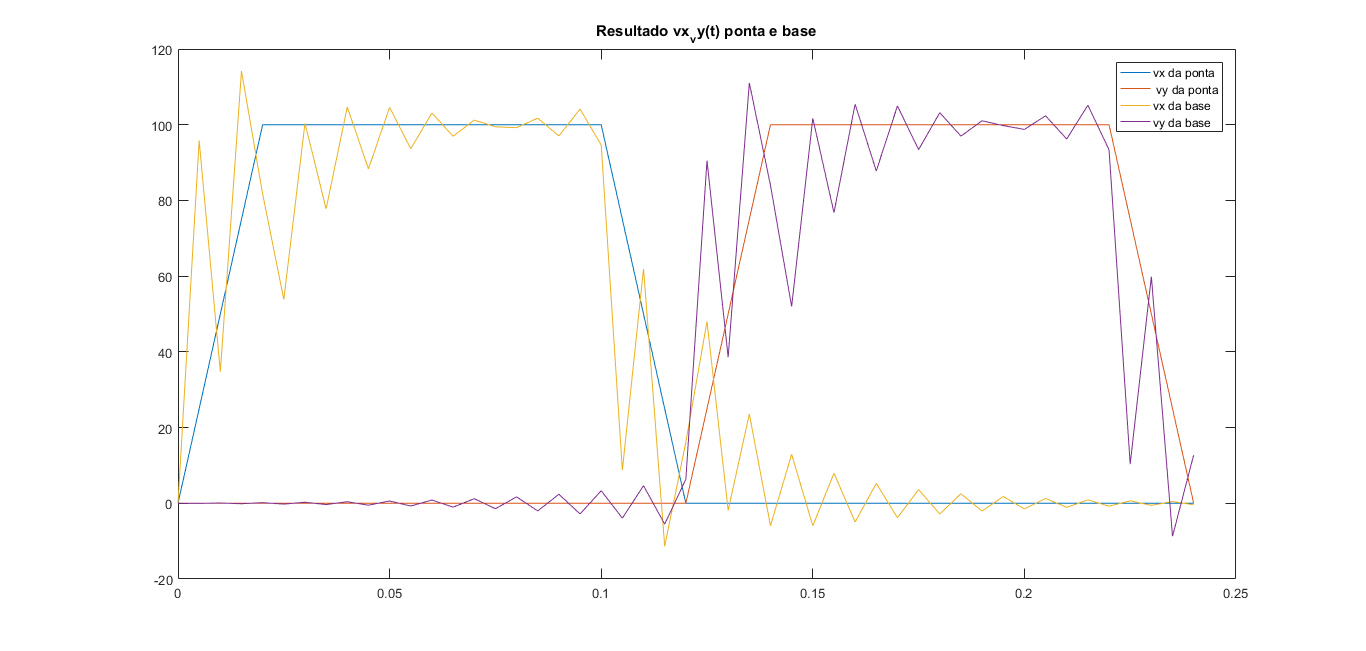
\includegraphics[scale=0.44]{Teste 5 B vels}
    \label{fig:t_5b_vels}
    \end{center}
\end{figure}

\begin{figure}[H]
    \begin{center}
    \caption{Caso 5C - Comportamento no tempo das velocidades em x e y da ponta e da referência}
    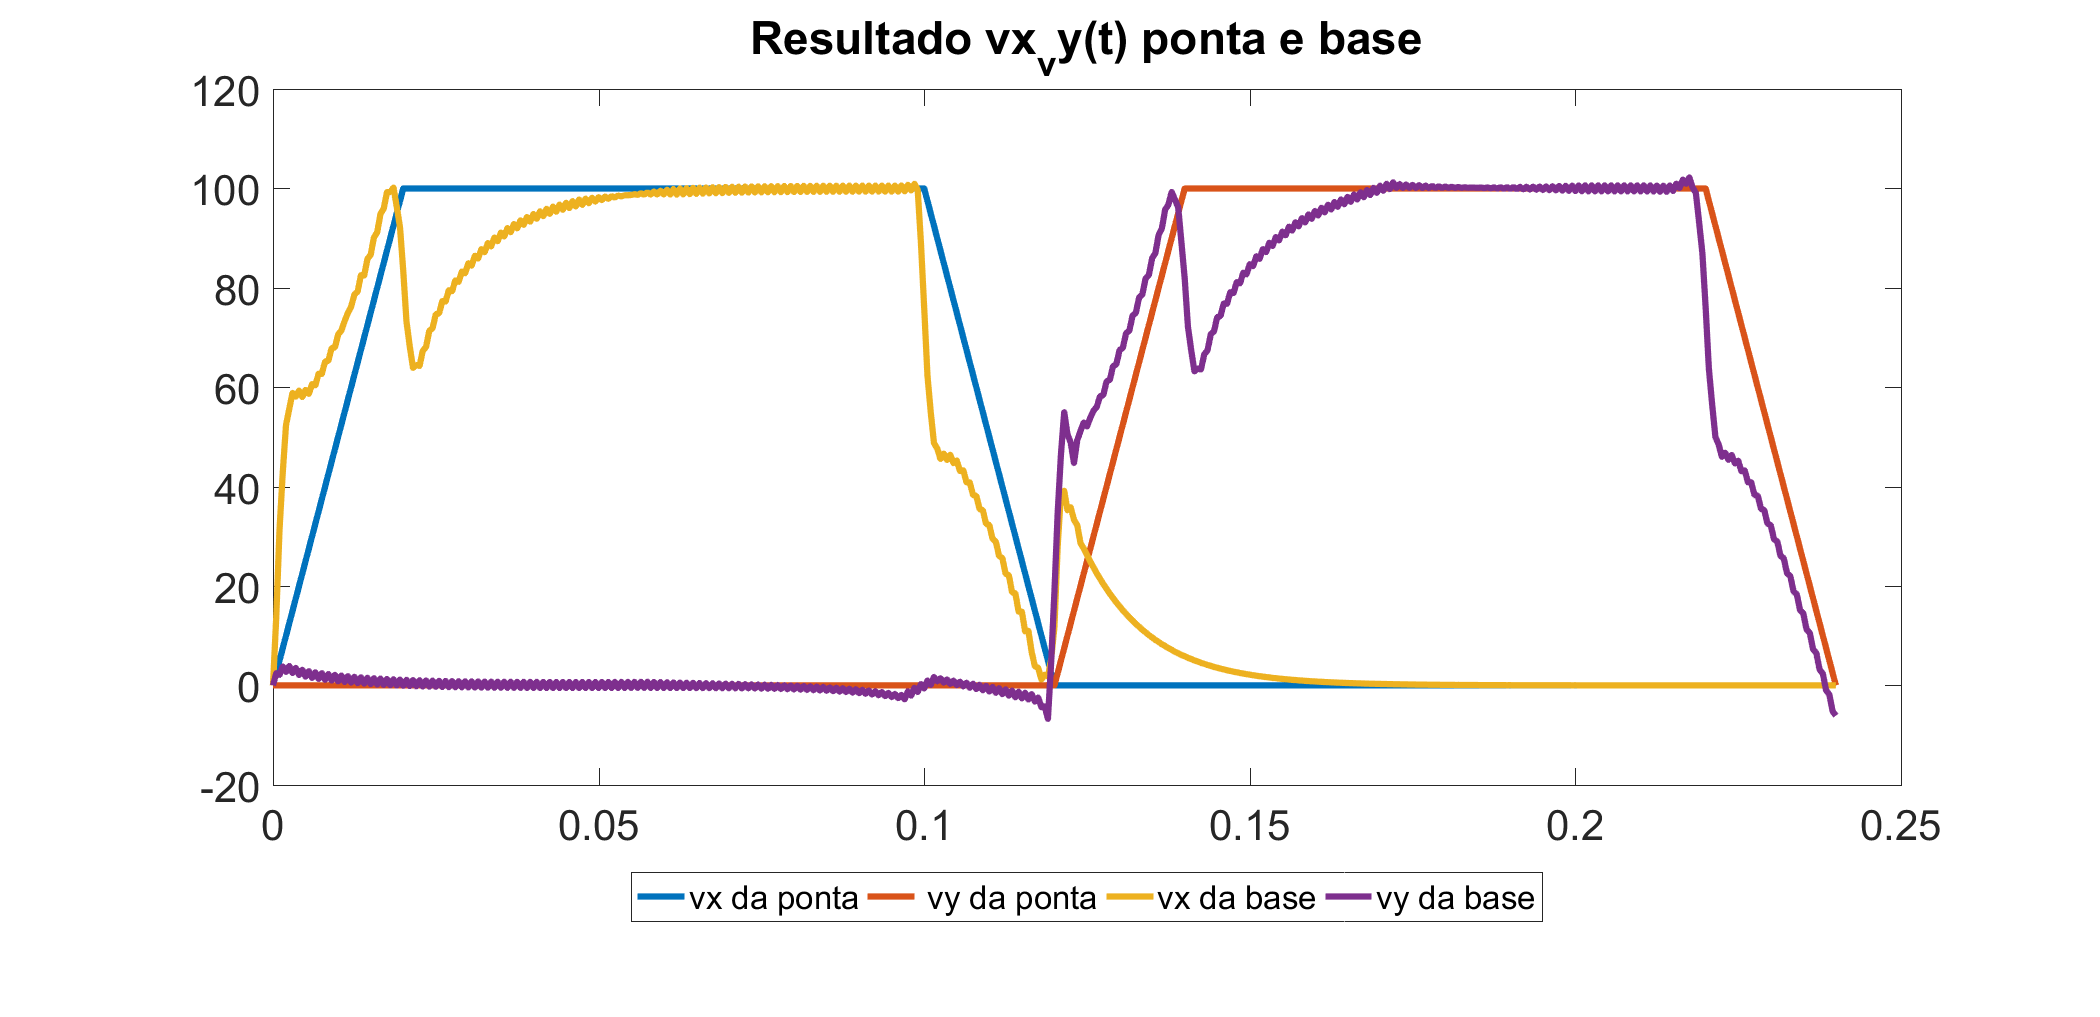
\includegraphics[scale=0.44]{Teste 5 C vels}
    \label{fig:t_5c_vels}
    \end{center}
\end{figure}

\begin{figure}[H]
    \begin{center}
    \caption{Caso 5A - Comportamento no tempo dos deslocamentos em x e y da ponta e da referência}
    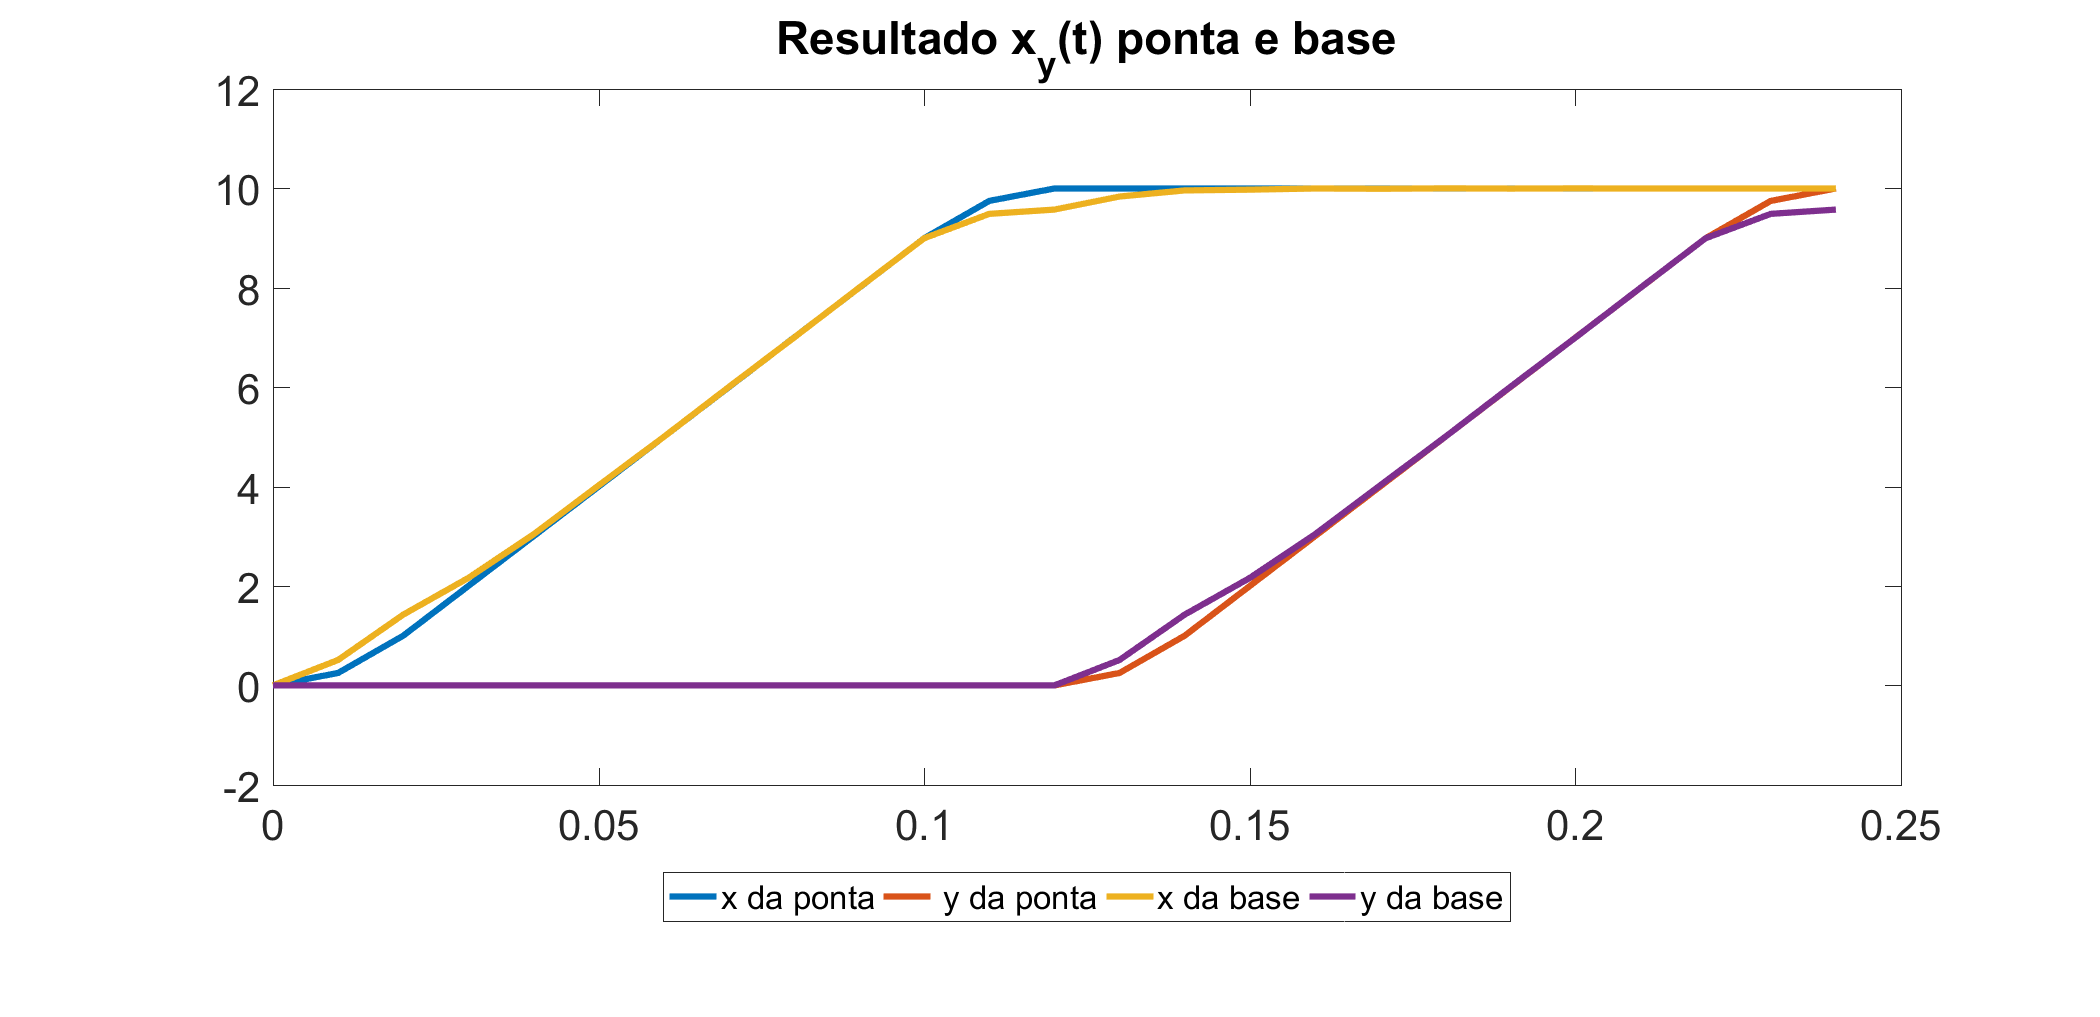
\includegraphics[scale=0.44]{Teste 5 A des}
    \label{fig:t_5a_des}
    \end{center}
\end{figure}

\begin{figure}[H]
    \begin{center}
    \caption{Caso 5B - Comportamento no tempo dos deslocamentos em x e y da ponta e da referência}
    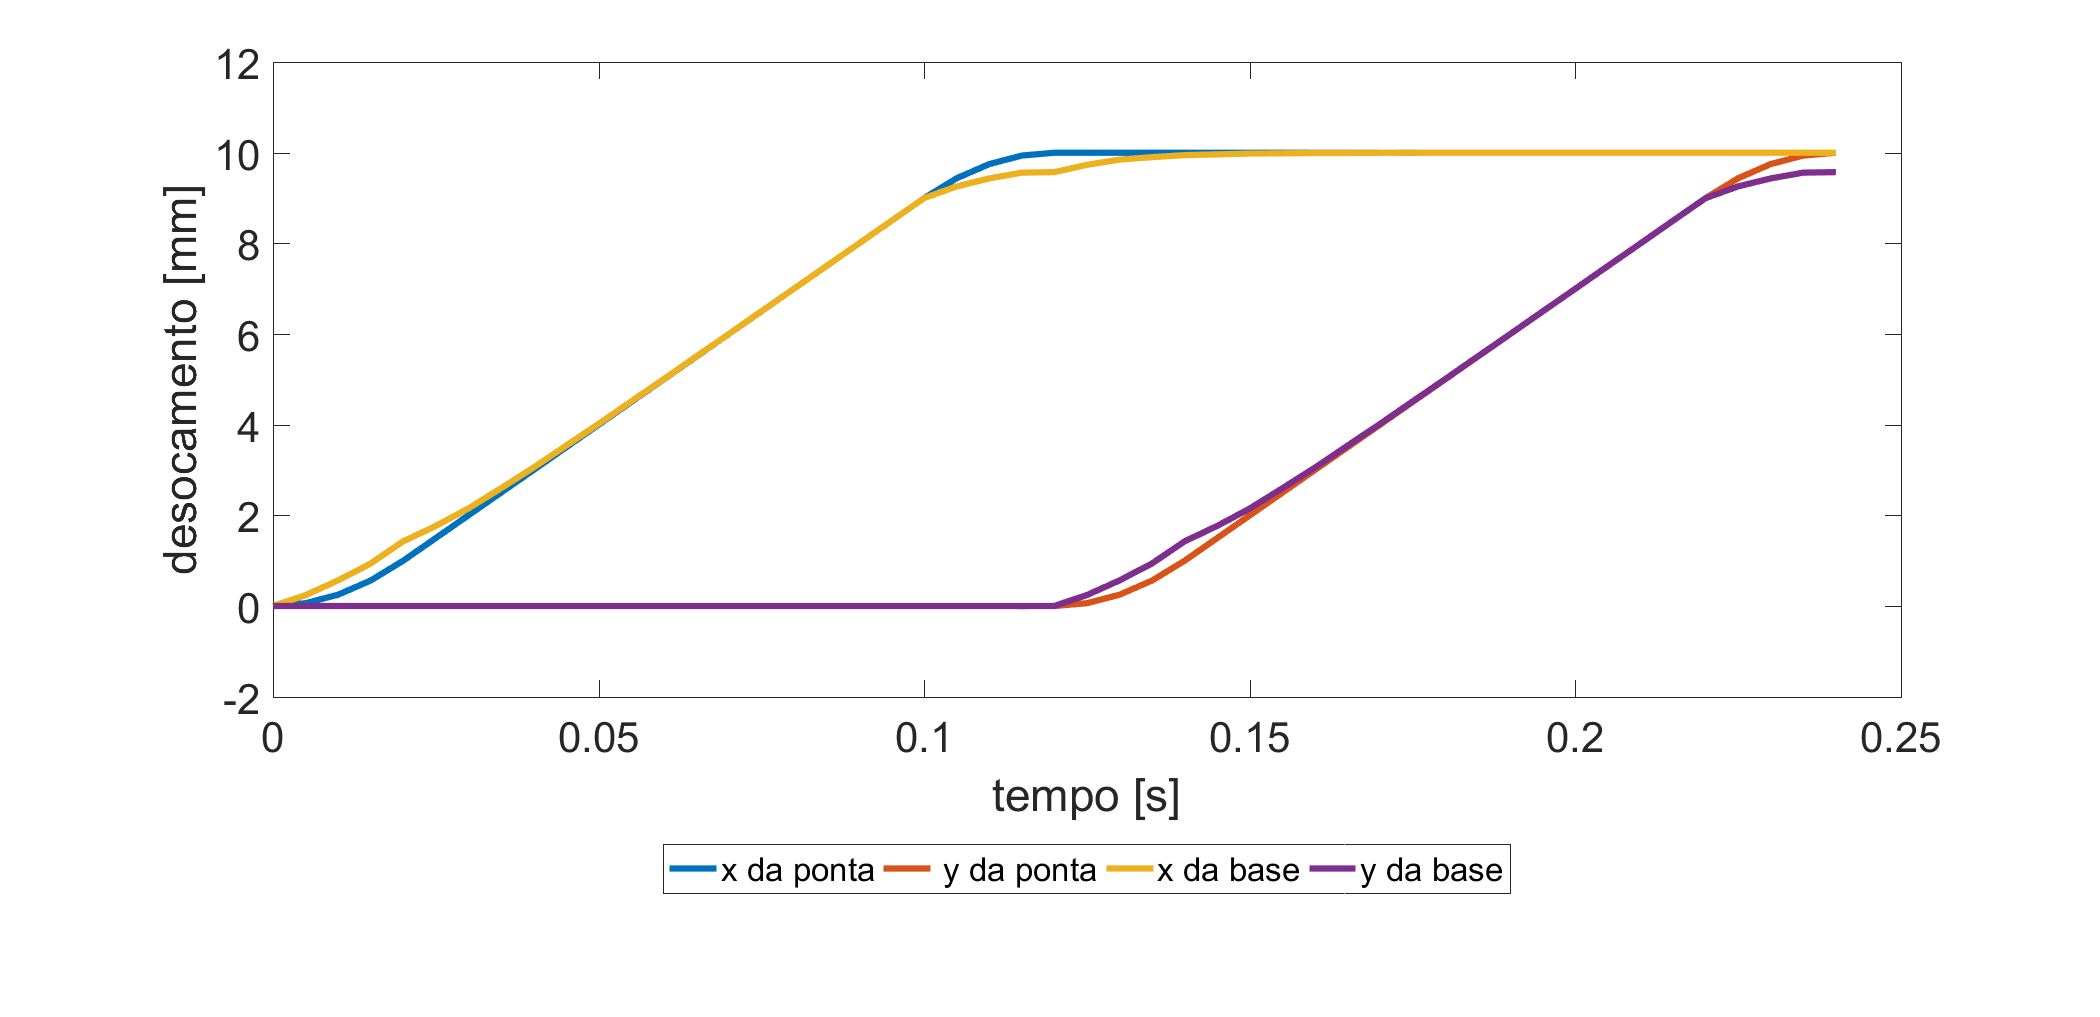
\includegraphics[scale=0.44]{Teste 5 B des}
    \label{fig:t_5b_des}
    \end{center}
\end{figure}

\begin{figure}[H]
    \begin{center}
    \caption{Caso 5C - Comportamento no tempo dos deslocamentos em x e y da ponta e da referência}
    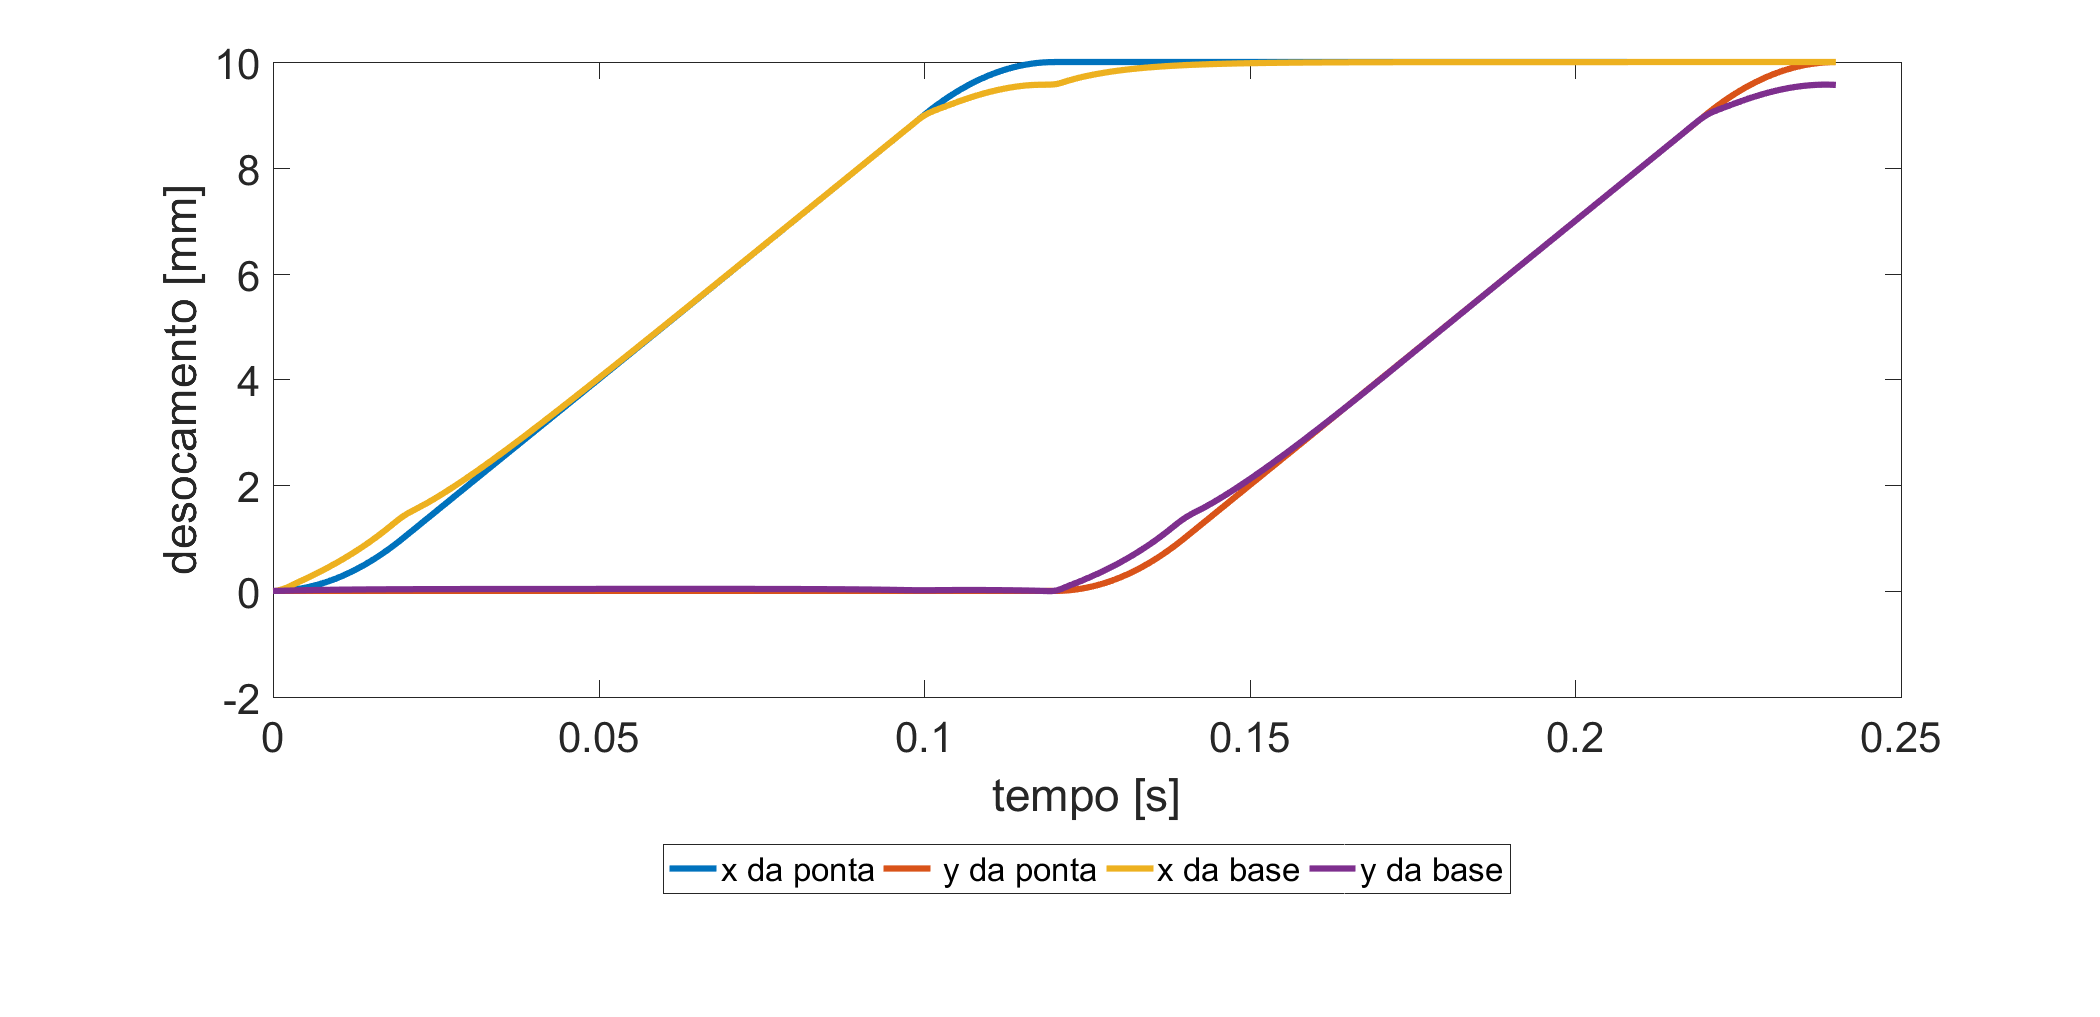
\includegraphics[scale=0.44]{Teste 5 C des}
    \label{fig:t_5c_des}
    \end{center}
\end{figure}

Podemos notar também o impacto na velocidade e facilidade de se convergir, podendo ser observado na figura \ref{fig:t_5_viab}, assim
como os tempos de simulação $0,7 s$, $3 s$ e $279 s$ para os Casos A, B e C respectivamente. Além do tamanho dos vetores que extá diretamente relacionado,
respectivamente em 25, 49 e 481 para os Casos A, B e C.

\begin{figure}[H]
    \begin{center}
    \caption{Caso 5 - Num de fun x Viabilidade}
    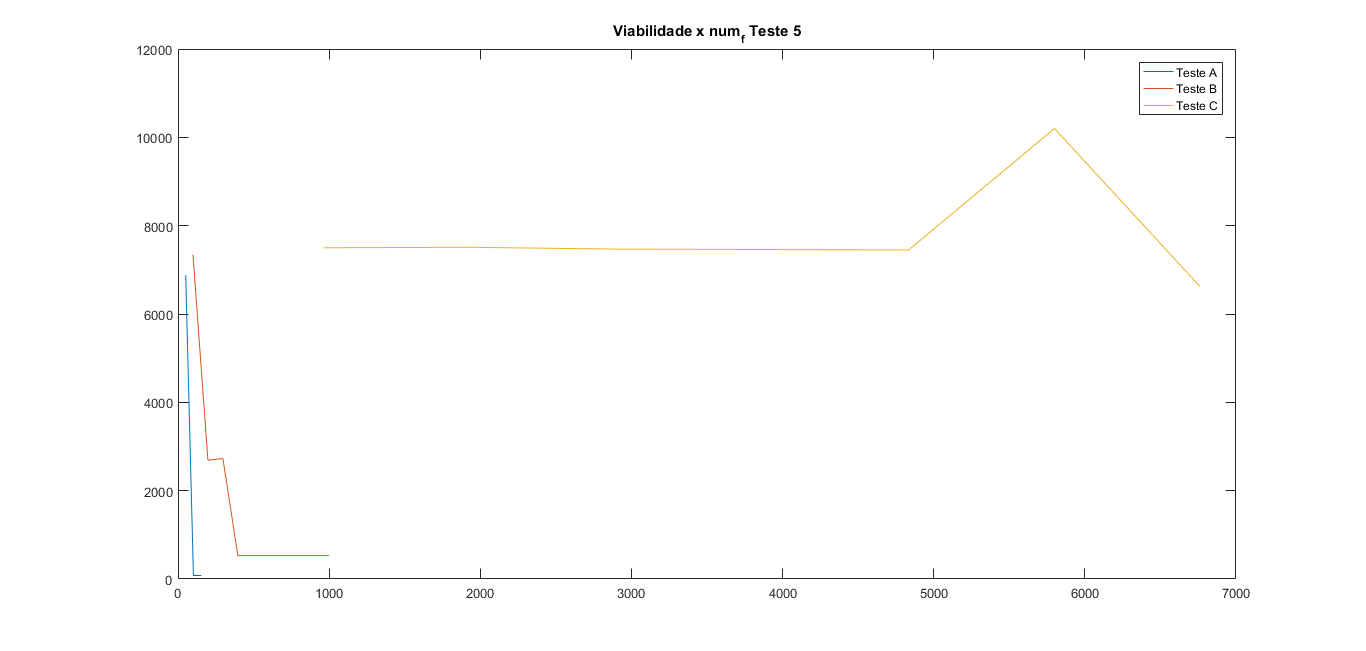
\includegraphics[scale=0.44]{Teste 5 Viabilidade}
    \label{fig:t_5_viab}
    \end{center}
\end{figure}

\section{Considerações futuras}
\subsection{Combinação com outros algoritmos}
Uma possível abordagem a ser explorada utilizando a ideia do método deste trabalho é a sobreposição de algoritmos, onde
um método referenciado em uma planta do sistema poderia buscar remover uma parcela das vibrações, atuando de forma estagiada,
com a participação de um método como \textit{InputShaping} para atacar as vibrações remanescentes.

\subsection{\textit{Tuning}}
Uma possibilidade que o tipo de método abordado neste trabalho oferece é a capacidade de otimizar, de maneira
semelhante aos mapas de injeção eletrônica para carros, os parâmetros da planta para uma determinada posição.
Assim, oferecendo a capacidade de se ajustar em grande nível de detalhe as peculiaridades do sistema, podendo até
construir a malha utilizando sensores, semelhantemente a rotinas de configuração de \textit{InputShaping} que amostram
o comportamento em frequência no ponto central da impressora. Considerando também que a utilização desse tipo de malha,
teria pouco impacto computacional.


